\documentclass[11pt,letterpaper]{article}
\usepackage[margin=0.88in,headheight=15pt,footskip=27pt]{geometry}
\usepackage{fontspec}
\setmainfont{lmroman10-regular.otf}[BoldFont=lmroman10-bold.otf,
 ItalicFont=lmroman10-italic.otf,BoldItalicFont=lmroman10-bolditalic.otf]
\setsansfont{lmsans10-regular.otf}[BoldFont=lmsans10-bold.otf,
 ItalicFont=lmsans10-oblique.otf,BoldItalicFont=lmsans10-boldoblique.otf]
\setmonofont{DejaVu Sans Mono}[Scale=0.80]
\usepackage{amsmath,amssymb,amsthm,mathtools,stmaryrd}
\usepackage{microtype}
\usepackage{booktabs,longtable,tabularx,array}
\usepackage{graphicx,xcolor,tikz}
\usetikzlibrary{arrows.meta,positioning,fit,calc}
\usepackage{enumitem,fancyhdr,titlesec,needspace}
\usepackage{fvextra}
\usepackage[most]{tcolorbox}
\usepackage{xurl,hyperref,bookmark}
\usepackage{caption}
\definecolor{ink}{HTML}{202820}
\definecolor{accent}{HTML}{435A46}
\definecolor{muted}{HTML}{626962}
\definecolor{soft}{HTML}{F3F4ED}
\definecolor{rule}{HTML}{B7BEB1}
\hypersetup{colorlinks=true,linkcolor=accent,citecolor=accent,urlcolor=accent,
 pdftitle={Leant2: Lean-Native Synthesis of Programs and Their Contracts},
 pdfauthor={OpenAI},pdfsubject={Architecture, algorithms, and reproducible prototype experiments}}
\urlstyle{same}
\setlength{\parindent}{0pt}
\setlength{\parskip}{5pt plus 1pt minus 1pt}
\setlength{\emergencystretch}{3em}
\setlist{nosep,leftmargin=1.6em,topsep=4pt}
\setcounter{tocdepth}{2}
\setcounter{secnumdepth}{3}
\titleformat{\section}{\Large\sffamily\bfseries\color{accent}}{\thesection}{0.6em}{}
\titleformat{\subsection}{\large\sffamily\bfseries}{\thesubsection}{0.6em}{}
\titleformat{\subsubsection}{\normalsize\bfseries}{\thesubsubsection}{0.6em}{}
\titlespacing*{\section}{0pt}{18pt}{7pt}
\titlespacing*{\subsection}{0pt}{12pt}{4pt}
\pagestyle{fancy}\fancyhf{}
\fancyhead[L]{\small\sffamily Leant2\enspace /\enspace Technical design}
\fancyhead[R]{\small\sffamily\thepage}
\renewcommand{\headrulewidth}{0.3pt}
\fancypagestyle{plain}{\fancyhf{}\fancyfoot[C]{\thepage}\renewcommand{\headrulewidth}{0pt}}
\newcommand{\code}[1]{\texttt{\detokenize{#1}}}
\newcommand{\Expr}{\code{Expr}}
\newcommand{\MetaM}{\code{MetaM}}
\newcommand{\Sort}{\mathsf{Sort}}
\newcommand{\Prop}{\mathsf{Prop}}
\newcommand{\Type}{\mathsf{Type}}
\newcommand{\G}{\Gamma}
\newcommand{\E}{\mathcal E}
\newcommand{\Q}{\mathcal Q}
\newcommand{\C}{\mathcal C}
\newcommand{\R}{\mathcal R}
\newcommand{\Budget}{\mathcal B}
\newcommand{\FV}{\operatorname{FV}}
\newcommand{\Comp}{\operatorname{Comp}}
\newcommand{\Obs}{\operatorname{Obs}}
\newcommand{\dom}{\operatorname{dom}}
\newcommand{\whnf}{\operatorname{whnf}}
\newcommand{\judges}{\vdash}
\newcolumntype{Y}{>{\raggedright\arraybackslash}X}
\newcolumntype{L}[1]{>{\raggedright\arraybackslash}p{#1}}
\DefineVerbatimEnvironment{Code}{Verbatim}{fontsize=\small,breaklines=true,
 breakanywhere=true,frame=leftline,framesep=7pt,rulecolor=\color{rule},
 xleftmargin=7pt,tabsize=2}
\AddToHook{env/Code/before}{\Needspace{6\baselineskip}}
\newtcolorbox{designbox}[1]{enhanced,breakable,colback=soft,colframe=rule,
 boxrule=0.5pt,arc=1mm,left=2.5mm,right=2.5mm,top=2mm,bottom=2mm,
 title={#1},coltitle=ink,colbacktitle=soft,fonttitle=\bfseries\sffamily}
\newtheorem{proposition}{Proposition}[section]
\newtheorem{invariant}[proposition]{Invariant}
\newtheorem{definition}[proposition]{Definition}
\theoremstyle{remark}\newtheorem{remark}[proposition]{Remark}
\newcommand{\repoLeant}{\href{https://github.com/VladimirReshetnikov/Leant/tree/6bf05ad78c467989e68290f2d08bbed40802d485}{Leant, revision 6bf05ad7}}
\newcommand{\repoDjex}{\href{https://github.com/VladimirReshetnikov/Djex/tree/e8778f4ebd63e1f9b9b410fa4de8d14a8a04c9e5}{Djex, revision e8778f4e}}
\begin{document}
\hypersetup{pageanchor=false}
\begin{titlepage}
\vspace*{0.45in}
{\sffamily\small\color{accent} ARCHITECTURE\quad /\quad ALGORITHMS\quad /\quad EXPERIMENTS}\par
\vspace{0.45in}
{\Huge\sffamily\bfseries Leant2}\par
\vspace{0.15in}
{\LARGE\sffamily Lean-Native Synthesis of\par Programs and Their Contracts}\par
\vspace{0.32in}
{\large A technical design for a Lean-only successor\par to Leant and Djex}\par
\vspace{0.3in}
{\normalsize Prepared for Vladimir Reshetnikov\par September 17, 2026}\par
\vspace{0.45in}
\begin{abstract}
We propose a program synthesizer whose semantic language is Lean itself: exact
universe-polymorphic expressions, dependent telescopes, inductive families,
class evidence, and behavioral propositions. Its central operation is not
``inhabit a simplified type, then test the rendering,'' but a transactional
search for a program and a proof of its exact contract. The search combines
bidirectional term construction, dependency-aware proof obligations,
recursor-derived recursion schemas, library specifications, counterexample
guidance, and optional certified theory solvers. A separate acceptance path
checks closed declarations in the kernel and records their assumptions.

The design specifies the boundaries that make such a system implementable:
which state must be backtracked, how polymorphic applications are instantiated,
how dependent elimination creates motives and transports, when an abstraction
may prune a sketch, and why finite-example equivalence must not permanently
delete alternatives. It also gives an implementation sequence and a benchmark
protocol for measuring practical coverage without changing the original goals.

Two accompanying experiments ground the proposal. A small Lean-native search
engine passed fifteen complete synthesis cases and two supplied elimination
skeletons with synthesized branches on Lean 4.34.0. A finite list-fold experiment
compares ordinary and length-guided counterexample search; separate Lean proofs
verify the length abstraction and the exact selected reverse program. These
experiments validate mechanisms, not a completed Leant2 implementation or a
measured success rate on arbitrary Lean projects.
\end{abstract}
\vfill
{\small\color{muted} Source snapshots: Leant \code{6bf05ad7}; Djex \code{e8778f4e}.\par
Experimental checker: Lean 4.34.0 via AXLE, invoked through Wolfram Language.\par
The archive includes source, experiment scripts, results, and check summaries.}
\end{titlepage}
\hypersetup{pageanchor=true}
\pagenumbering{roman}
{\small\linespread{0.9}\selectfont\setlength{\parskip}{0pt}
\tableofcontents}
\newpage
\pagenumbering{arabic}
\section{The architectural decision}

\begin{designbox}{Recommendation}
Build Leant2 as a Lean-native, specification-directed synthesizer over exact
Lean expressions. Keep an explicit, resumable search-control representation,
but do not introduce another authoritative type language. Search jointly for
computational terms and their contract proofs; accept only their kernel-checked
closure in the original environment. Make recursion schemas, typed library
specifications, and behavioral guidance first-class parts of the engine.
\end{designbox}

A language change by itself does not create a stronger synthesizer. Translating
Djinn and Exference into Lean while retaining their effective search language
would simplify deployment but preserve many of the limitations motivating this
project. Conversely, replacing every search node with an unconstrained call to
an existing proof tactic would give away control over computational alternatives,
termination, ranking, and specification-driven decomposition. Leant2 needs a
native semantic substrate \emph{and} a synthesis-specific search architecture.

The useful unit of work is a \emph{typed partial program together with all
obligations that constrain its completion}. Some obligations concern values,
some concern types or indices, and others concern behavior. A branch cannot
commit to a value merely because its type has been inhabited: a later proof
obligation can distinguish several values of that same type. This observation
will determine the state model, scheduler, cache design, and plugin protocol.

\subsection{What should survive from Leant and Djex}

The current repositories already do substantially more than erase Lean types
into Haskell arrows. Djex has distinct logical and heuristic search engines,
shared checked representations, and explicit evidence boundaries. Leant
preserves exact source associations for supported polymorphic applications and
checks generated candidates against Lean types. Its behavioral interface proves
a supplied proposition or its negation about the exact candidate, and reports
inconclusive outcomes separately. Those are strengths to retain, not defects to
``repair'' by renaming the implementation language~\cite{djex-architecture,leant-internals,leant-behavior}.

What should disappear is the obligation to make Lean's semantics fit a common
Haskell-facing type and expression vocabulary. The new search engine can inspect
an inductive declaration directly, carry a dependent family as an expression,
and let later arguments determine earlier implicit parameters. A first-class
value that is itself polymorphic needs no translation into an occurrence plan
whose meaning must subsequently be reconstructed in Lean.

The repository's earlier rewrite analysis already recommends Lean-native
preparation and a project-local worker, but retains a neutral synthesis
representation and confines metaprogramming state to boundaries~\cite{earlier-rewrite}.
This design makes a different, more specific choice: \emph{control state is
explicit and serializable; type meaning remains Lean-native}. Persistent branch
snapshots and replayable rule applications recover deterministic control without
requiring a second approximate type theory. This is not a proposal to replace an
explicit search tree with one opaque mutable tactic invocation.

The current indexing diagnostics also show that some missing results are
composition and ordering failures even when the needed components are
representable~\cite{indexing-diagnostic}. Leant2 therefore must improve search,
not merely increase the set of admissible types. The higher-rank examples in
our prototype are new mechanism tests, not reruns or resolutions of the
repositories' original indexing or two-universe acceptance queries.

\subsection{Scope of the intended coverage}

The first broad target is pure total programming and ordinary proof obligations:
polymorphic adapters; records and law-carrying structures; options, sums and
lists; user-defined inductives; indexed families; bounded indices; common
structural traversals; and programs assembled from specified library operations.
The second target is more demanding dependence: arithmetic casts, generalized
recursive motives, well-founded recursion, and relational contracts. Effects
require a semantics-specific contract layer rather than merely a term of type
\code{IO A}.

``A large fraction of practical types'' should be treated as an evaluation goal,
not a theorem or an unmeasured percentage. Two queries with identical outer
function types can differ radically in difficulty because their contracts,
providers, or local instances differ. Section~\ref{sec:evaluation} therefore
measures \emph{requests}, not just type strings.

\section{Requests, results, and semantic profiles}\label{sec:requests}

\subsection{A precise synthesis request}

Let a request be
\[
 \Q=(\E,U,\G,T,C,\R,\Pi,\Budget),
\]
where $\E$ is a frozen Lean environment, $U$ is the declared universe telescope,
$\G$ is the ordered local context including local definitions and instances,
$T$ is the exact requested type, $C$ is an optional contract, $\R$ is the
permitted construction inventory, $\Pi$ is a semantic and acceptance policy,
and $\Budget$ contains resource limits. We require
\[
 \E;U;\G\judges T:\Sort\,u,
 \qquad
 \E;U;\G,f:T\judges C(f):\Prop.
\]
Omitting the contract means $C(f)=\mathsf{True}$, not permission to guess what
the user intended from the name of the definition.

A successful result consists of a program $e$, a proof $p$, and any generated
auxiliary declarations $\Delta$ such that
\begin{equation}\label{eq:acceptance}
 \E,\Delta;U;\G\judges e:T,
 \qquad
 \E,\Delta;U;\G\judges p:C(e),
\end{equation}
and $\Delta$ is itself accepted in dependency order under policy $\Pi$. The
request fixes both the program type and the meaning of its predicate. Neither
may change when an instance is selected, a candidate is simplified, or a
counterexample is replayed.

For ordinary $T:\Type\,u$, the internal proof problem can often be expressed as
\code{{ f : T // C f }}. This is a useful implementation technique, not the
entire public representation. For arbitrary sort-polymorphic goals, generated
mutual declarations, or separate proof profiles, it is simpler to keep the term
and proof obligations explicitly paired and export two declarations. There is
no need to force every request into a particular dependent-pair encoding.

\subsection{Proposed Lean-only interfaces}

The following is a proposed interface, not syntax implemented by the included
microprototype:
\begin{Code}
synthdef chooseSecond : Nat -> Nat -> Nat
  satisfying fun f => forall x y, f x y = y
  using [Nat]

#synth (forall A : Type, A -> A)

def adapter : Input -> Output := by
  leant2 [allowedOperation1, allowedOperation2]

example : SomeProposition := by
  leant2?
\end{Code}

A term elaborator, a command elaborator, an interactive session, and an editor
code action should all prepare the same request object. The \code{?} form should
produce stable source or an explicit term that can be replayed without search.
A lower-level API should accept already elaborated expressions, avoiding a
string round trip for clients inside Lean.

Contracts are elaborated under a fresh local binder with the exact requested
type. Unknown contract names are errors, not inferred extra parameters. The
construction inventory and proof inventory are separate: a reference
implementation may legitimately appear in a specification without becoming a
permitted implementation provider. Attributes such as \code{@[leant2_provider]}
and \code{@[leant2_spec]} should expand into checked registry entries; they do
not make their contents trusted.

\subsection{Type-only, pointwise, and relational contracts}

Consider three distinct requests:
\begin{align*}
 &f:\operatorname{List}(A)\to\operatorname{List}(A),\\
 &f:\operatorname{List}(A)\to\operatorname{List}(A),
 &&\forall xs,\ |f(xs)|=|xs|,\\
 &f:\operatorname{List}(A)\to\operatorname{List}(A),
 &&\forall xs,\ f(xs)=\operatorname{reverse}(xs).
\end{align*}
Returning the empty list solves the first. Identity solves the second. Neither
solves the third. Penalizing ignored arguments or preferring a familiar
operation name is not a substitute for the missing contract.

When $C(f)$ is exactly $\forall x,Q(x,f(x))$, it can be useful to synthesize
\[
 g:\prod_{x:A}\{y:B(x)\mid Q(x,y)\},
 \qquad f(x)=g(x).\mathsf{val}.
\]
The projection proves the original contract. Conversely a known $f$ and its
pointwise proof provide such a $g$, so this transformation loses no solutions
up to the intended extensional behavior in this setting. The implementation
should register the transformation theorem rather than pattern-match its way
past a proof obligation.

Not every contract has this form. Monotonicity, injectivity, homomorphism laws,
noninterference, and algebraic laws can relate multiple executions. They remain
constraints on the shared global function. A pointwise output predicate cannot
silently replace them. A later relational-induction engine may decompose them,
but must reconstruct a proof of the original $C$.

\subsection{Computability and assumption policy}

The default profile should request a \emph{computable total definition}. A
separate mathematical profile may permit noncomputable existence-based
construction. In particular, a hypothesis \code{Nonempty A} is not an executable
value of type \code{A}. Allowing \code{Classical.choice} changes what can be
constructed; this must be visible in the request and receipt, not an automatic
fallback hidden behind a successful-looking answer. Lean's restrictions on
elimination from propositions are part of the semantics~\cite{lean-types}.

Likewise, proving a proposition about the logical meaning of a definition does
not verify arbitrary native replacements, foreign code, or unsafe runtime
implementations. The acceptance policy should distinguish logical dependencies,
computability, and runtime implementation dependencies. Lean's documentation
explicitly distinguishes these concerns for partial and unsafe definitions and
implementation replacements~\cite{lean-recursion}.

Useful profiles are \emph{constructive computation}, \emph{computation with an
explicit proof-axiom allowlist}, \emph{mathematical/noncomputable}, and
\emph{effectful with a chosen operational semantics}. There is no need to conflate
``uses \code{propext} in an erased correctness proof'' with ``uses classical
choice to produce the executable answer.'' Record both dependency closures.

\subsection{Result taxonomy}

\begin{tabularx}{\linewidth}{@{}L{0.24\linewidth}Y@{}}
\toprule
Result & Meaning \\
\midrule
Verified & A program and its exact original contract have passed the acceptance path. \\
Typed / residual & An explicitly requested sketch result: a term or partial program with named remaining obligations; not an implementation satisfying the contract. \\
Examples verified & The displayed finite conjunction is proved. No unproved universal property is implied. \\
Candidate refuted & A particular candidate has a checked counterexample or a proof of the negated contract. \\
Bounded exhaustion & No accepted candidate in the explored finite grammar and resource allowance; scope is reported. \\
Unknown / interrupted & Solver uncertainty, unsupported mechanism, timeout, cancellation, or worker failure. \\
Globally uninhabited & A kernel-checked proof of $T\to\mathsf{False}$, or an equivalent appropriate emptiness assertion, in the stated context. \\
\bottomrule
\end{tabularx}

For a data type $T$, writing $\neg T$ is not the right Lean proposition: $T$ is
not itself a proposition. More subtly, a Kripke countermodel showing that a
propositional formula is not derivable in intuitionistic logic is not generally
a Lean proof of its negation. Leant2 may report a certified \emph{fragment
non-derivability} result with its explicit scope; it must not promote it to a
semantic emptiness theorem in the full ambient environment.

\section{Subsystems and the one semantic authority}\label{sec:architecture}

\begin{figure}[ht]
\centering
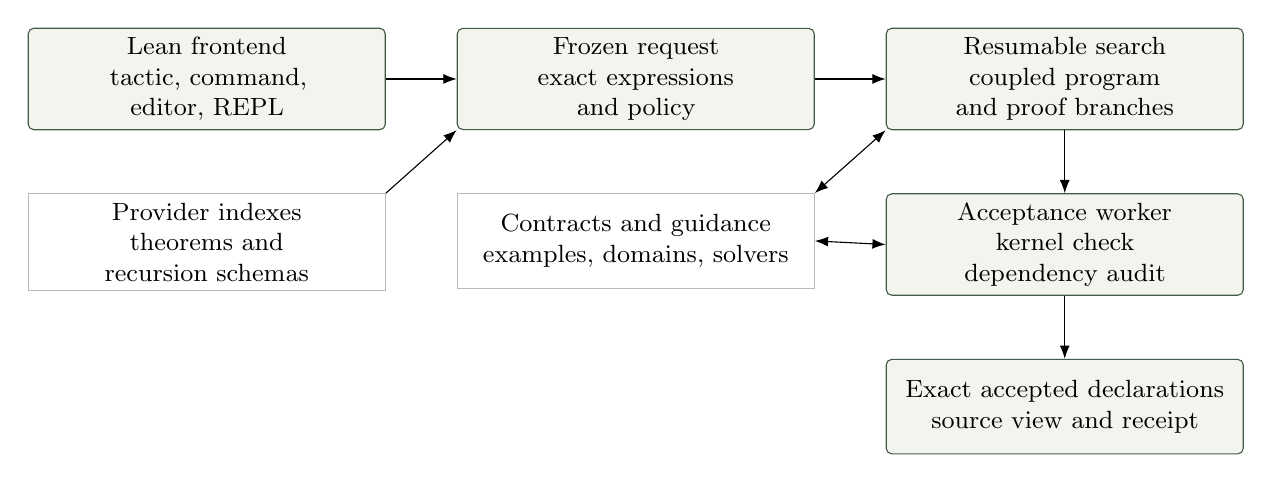
\begin{tikzpicture}[node distance=8mm and 9mm,>=Latex,
 b/.style={draw=accent,rounded corners=2pt,fill=soft,align=center,
 text width=43mm,minimum height=12mm,font=\small},
 s/.style={draw=rule,align=center,text width=43mm,minimum height=12mm,font=\small}]
\node[b] (front) {Lean frontend\\tactic, command, editor, REPL};
\node[b,right=of front] (request) {Frozen request\\exact expressions\\and policy};
\node[b,right=of request] (search) {Resumable search\\coupled program\\and proof branches};
\node[s,below=of front] (lib) {Provider indexes\\theorems and\\recursion schemas};
\node[s,below=of request] (guide) {Contracts and guidance\\examples, domains, solvers};
\node[b,below=of search] (check) {Acceptance worker\\kernel check\\dependency audit};
\node[b,below=of check] (output) {Exact accepted declarations\\source view and receipt};
\draw[->] (front)--(request); \draw[->] (request)--(search);
\draw[->] (lib.north east)--(request.south west);
\draw[<->] (guide.east)--(check.west);
\draw[<->] (guide.north east)--(search.south west);
\draw[->] (search)--(check); \draw[->] (check)--(output);
\end{tikzpicture}
\caption{The semantic core stays in Lean. External tools propose information;
only the acceptance path publishes verified results. The diagram is a logical
component view, not a requirement for one process per box.}
\end{figure}

\subsection{Core packages}

\code{Leant2.Core} should own request identities, policies, typed obligations,
and result envelopes. \code{Leant2.LeanBridge} should wrap version-sensitive
metaprogramming operations: telescope opening, application, cases, recursor
inspection, local abstraction, and checked declaration admission.
\code{Leant2.Search} should own explicit branch state, rule cursors, budgets,
and scheduling. \code{Leant2.Providers} should manage term and theorem indexes.
\code{Leant2.Contracts} should implement decomposition and proof orchestration.
\code{Leant2.Recursion} should derive typed recursive schemas.
\code{Leant2.Domains} should host optional abstractions, testing codecs, and
certified theory translations. \code{Leant2.Accept} should own final closure,
replay, audits, and export.

The dependency direction matters: search may call the acceptance facade, but a
checker must not rely on a search node's claim that it has been solved. A domain
plugin may inspect an exact expression or its own certified reification. It
must not replace the request type with the domain's abstraction. Presentation
should consume accepted records rather than construct them.

\subsection{Two representations, but only one type theory}

Lean expressions are the semantic representation. A second representation is
still useful for \emph{search actions}: introduce this binder; apply this exact
provider with these choices; split this scrutinee; instantiate this recursive
schema; request this proof method. Such a plan is a small replayable recipe
whose successful execution produces an expression and obligations.

This control language is not a second typing authority. Its annotations contain
exact Lean expressions, references to immutable request-local objects, or
closed templates checked when instantiated. A domain-specific reified AST is
also legitimate, as in our list-fold experiment, provided its interpretation
into Lean and its analysis theorems are explicit. The prohibition is against
making an approximation silently authoritative for all Lean types.

\subsection{Worker and controller}

A project-local worker is built with the project's Lean toolchain and imports.
It owns expressions, environments, elaboration, and search. A long-lived
controller, also implementable in Lean, owns sessions, progress, cancellation,
and durable requests. The tactic frontend can run directly in the current
worker; the standalone frontend should not load arbitrary project artifacts
into a globally built executable. This preserves the earlier rewrite analysis's
useful toolchain-isolation boundary~\cite{earlier-rewrite}.

Cross-process messages contain source requests, checked exported declarations,
or a versioned serialized plan with an exact environment identity. Raw
\code{MVarId} and \code{FVarId} values never become durable identifiers. A worker
restart invalidates its ephemeral handles. An undo produces a new environment
generation even if pretty-printed declarations look unchanged.

\section{The search state is a dependency graph}\label{sec:state}

\subsection{A branch contains more than a goal}

A minimal production branch should contain the following conceptual fields:
\begin{Code}
Branch := {
  requestId, environmentGeneration, branchId,
  rootProgram, rootContractProof,
  metaSnapshot, elaboratorSnapshot, declarationDelta,
  pendingObligations, dependencyGraph, blockedConstraints,
  recursionCapabilities, exampleBankVersion,
  domainFacts, decisionTrail, ruleCursors,
  accumulatedCost, resourceCharges
}
\end{Code}
This is a schema, not an assertion that these are stable Lean API record names.
The snapshots must include all state that the chosen rule can mutate. A purely
\MetaM{} rule can use a metaprogramming snapshot; a command-level rule creating
auxiliary declarations needs an environment/elaborator transaction as well.
Restoring only the current list of goals is insufficient. Lean's metavariable
operations and unification can assign information that later operations
observe~\cite{meta-book,lean-apply}.

Each obligation has a kind, a target expression, its owning local context, a
read/write set of reachable metavariables, dependencies, and an origin. Kinds
include computational value, type or universe choice, instance evidence,
index equality, contract proof, termination proof, and reconstruction check.
The distinction guides scheduling; it does not create different logical
notions of truth.

Connect two obligations when either can assign a metavariable reachable from
the other, including metavariables in local declaration types, local values,
instance arguments, or universe expressions. Transitive connected components
are \emph{coupled clusters}. Assignment can create or remove dependencies, so
the graph must be incrementally refreshed. A static syntactic list of initial
free metavariables is not enough.

\subsection{The fundamental continuation invariant}

Suppose a constructor creates holes $h_1:A$ and $h_2:P(h_1)$. It is incorrect to
run a solver for $h_1$, retain its first inhabitant, and only then begin an
independent solver for $h_2$. Failure of $P(h_1)$ must be able to revisit the
choice of $h_1$. The same applies to a provider's type parameter, a class
instance, an inductive index, or a recursive helper's invariant.

\begin{invariant}[Continuation ownership]\label{inv:continuation}
An alternative is successful only if its entire coupled continuation is
successful. Every decision that can affect a remaining obligation retains a
backtracking point until the cluster is accepted or deliberately suspended.
\end{invariant}

For example, the subtype
\[
 \{f:\mathbb N\to\mathbb N\to\mathbb N\mid f(11,29)=29\}
\]
first asks for a function and then for a proof. Returning the first argument is
type correct. Its proof obligation fails. Returning the second argument is then
tried and its equality reduces to reflexivity. The included Lean experiment
implements precisely this continuation discipline. It does not use a special
rule recognizing the words ``choose second.''

\subsection{Transactional rule execution}

A robust rule application follows this protocol:
\begin{Code}
tryRule(branch, rule):
  checkpoint := snapshotAllStateWritableBy(rule)
  result := rule.nextAlternative(branch)
  if result is an ordinary inapplicability:
      restore checkpoint; return NotApplicable
  if result is interruption or exhausted global resources:
      restore checkpoint; propagate status
  if result is a new typed branch:
      compute new dependencies and branch-local obligations
      retain checkpoint/decision for its coupled continuation
      return SuspendedBranch(result)
\end{Code}

Unexpected plugin exceptions should become diagnostics, not silently be treated
as a logical dead end. The microprototype intentionally has a much smaller
exception policy; production code should distinguish unification mismatch,
unsupported term form, local proof timeout, cancellation, internal error, and
resource exhaustion. In particular, repeated catching of heartbeat exhaustion
must not create a loop that appears to make search progress.

Parallel branches own independent snapshots and solver frames. Sharing
immutable expressions and environment data is useful; sharing a writable
metavariable context is not. Exporting a result from one branch to another
requires an abstracted template with explicit parameters and a fresh replay,
not copying a live expression containing foreign metavariable identifiers.

\section{Bidirectional construction over Lean expressions}\label{sec:bidirectional}

\subsection{Two judgments and a suspended constraint store}

The engine alternates between checking a proposed shape against an expected
type and inferring the type of a neutral expression:
\[
 \G\judges e\Leftarrow T
 \qquad\text{and}\qquad
 \G\judges n\Rightarrow T.
\]
A neutral expression is typically a local variable or permitted constant
applied to an argument spine, possibly followed by projections. These are
search judgments; the actual resulting term is still checked by Lean.

The expected type drives introductions. The head of an available term drives
eliminations. A suspended constraint store records equations that cannot yet be
resolved without a missing argument or instance. It is important not to
interpret ``blocked'' as ``false.'' A rule that only increases the number of
unconstrained metavariables should be charged a cost and postponed behind rules
that expose structure.

\subsection{Introduction rules}

For a dependent function, introduce a rigid local parameter:
\[
 \frac{\G,x:A\judges e\Leftarrow B(x)}
      {\G\judges (\lambda x.e)\Leftarrow \prod_{x:A}B(x)}.
\]
The binder retains its type, visibility, and instance status. A universe or
type parameter belonging to the original theorem is a rigid parameter; the
synthesizer is not allowed to specialize it to \code{Nat} merely because that
makes the current example executable.

For a dependent pair, create the witness hole before its dependent field:
\[
 \frac{\G\judges a\Leftarrow A\quad
       \G\judges b\Leftarrow B(a)}
      {\G\judges (a,b)\Leftarrow \sum_{x:A}B(x)}.
\]
Both holes remain coupled. A record constructor generalizes this rule: its
fields are processed in the actual constructor telescope, including inherited
fields and proof fields. Record synthesis must not assume that the displayed
field order is a list of independent goals.

For an inductive target $I\,\bar p\,\bar i$, inspect the environment's constructor
information. Freshen the constructor's universe levels, instantiate its
parameters, and unify its result with the target. The remaining fields become
obligations in that same transaction. A constructor whose index equation is
inconsistent can be rejected. A constructor whose equation is merely blocked
must remain available, or be recorded as a bounded search omission rather than
a proof of impossibility.

Functions and records should not always be expanded immediately. An existing
local function may solve the whole goal more cheaply than an eta expansion.
Keep a cheap exact-term lane before decomposing. Conversely, a cheap inhabitant
must not suppress later contract-sensitive alternatives. Introductory focusing
is an ordering discipline; a claim that a rule is irrevocably safe needs to
account for the whole contract and the chosen equivalence/cost notion.

\subsection{Application-spine search}\label{sec:spines}

For a candidate head $h$, do not enumerate complete argument tuples blindly.
Use a demand-directed spine algorithm:
\begin{Code}
applyHead(h, expectedType, branch):
  freshen all universe parameters of this occurrence of h
  inspect the exact dependent telescope of typeOf(h)
  enumerate admissible partial-application lengths lazily
  create fresh argument holes in telescope order
  constrain the instantiated result against expectedType
  propagate assignments through argument types and local instances
  discharge determined instance and proof arguments cheaply
  suspend blocked constraints; prioritize informative arguments
  yield the application and its entire coupled continuation
\end{Code}

Lean's \code{MVarId.apply} already provides much of the basic mechanism,
including result matching, argument metavariables, and instance processing.
The prototype uses its exact-unification configuration and requests
\code{newGoals := .all}, rather than relying on a UI-oriented goal order that
may hide dependent goals~\cite{lean-apply}. The production wrapper must also
account for delayed metavariables, universe constraints, and obligations
created by any later elaboration step. ``The tactic returned no goals'' is not
the final acceptance test.

A head may have a type such as
\[
 \prod_{A:\Type u}(x:A)\,
 \prod_{B:A\to\Type v}(k:\prod_{a:A}B(a)),\ B(x).
\]
There is no meaningful global split into ``all type arguments first, then all
value arguments.'' Instantiation follows the actual telescope. Solving $x$
may constrain $A$; the expected result may constrain $B$; a class obligation
may later determine an output parameter. All those assignments belong to one
branch.

Index providers by a conservative approximation to their result heads, arity,
and binder shape, but include fallback buckets for variable-headed and
reducible results. An index is allowed to return extra candidates. Omitting a
candidate for speed is a heuristic restriction that must not contaminate a
completeness claim. A small local context should be searched before the global
inventory, without becoming an absolute restriction on the latter.

\subsection{Higher-rank arguments and universes}

A polymorphic callback is simply an argument whose type is itself a dependent
function type. When the expected argument is
\code{(A : Type u) -> A -> A}, introduction creates a rigid $A$ and then a rigid
$x:A$; using $x$ completes that callback. A provider that accepts such a callback
can therefore be applied without translating it to a monotype or inventing a
new representation for rank two, three, or four.

Each occurrence of a polymorphic global receives fresh level metavariables.
The original query's universe parameters remain fixed. Two uses need not share
a fresh level assignment merely because they share a declaration name, while
correlations explicitly present in one application telescope must be preserved.
The prototype's independent-$u$ and independent-$v$ callbacks test one instance
of this distinction.

Lean's universe discipline must remain in force. Treating a polymorphic type
as an argument is not permission to identify \code{Type u} with an arbitrarily
large universe or to make \code{Type} impredicative. \code{Prop} has a distinct
impredicative role; nested quantification at \code{Type} still has its actual
sort~\cite{lean-types}. Lean is also noncumulative: a type at one universe does not automatically
inhabit every larger universe. An explicit lift is a typed construction, not
a numeric relaxation of a level constraint. No fixed list of universe levels
should appear in the semantic kernel of Leant2. A bounded list may be used in an explicitly
heuristic instantiation proposal lane.

Some type-valued holes remain genuinely underconstrained. Search them using
expected-type information, subexpressions of the local/provider types,
instantiation templates, and bounded enumeration of well-sorted type
expressions. Avoid committing every such hole to the first visible type.
Return an explicit request for a sketch annotation only as an interactive aid;
ordinary bounded search can still return an honest unknown.

\subsection{Unification is a service, not a completeness oracle}

Direct use of Lean removes the need to reimplement its definitional equality,
but does not make higher-order inference complete. The engine should classify
constraints into deterministic progress, blocked progress, speculative
assignment, and mismatch. A failed unification attempt is usually an
inapplicable rule alternative, not a theorem that no inhabitant exists.

In the first implementation, use Lean's standard unifier transactionally and
revisit alternative heads, argument orders where permitted, and explicit
instantiation hints. Later, add a bounded higher-order proposal layer:
pattern-like metavariable applications are solved first; remaining flexible
heads may be instantiated with small lambda/projection/application templates.
Every proposal returns to Lean for checking. This is preferable to building a
second, subtly incompatible conversion procedure.

Opaque constants, casts, and reducibility settings require particular care.
Use weak-head reduction to expose the structure needed by the current rule;
do not repeatedly normalize every expression in the environment. A reduction
cache key includes its transparency mode and relevant metavariable assignments.
Forcing an opaque provider to unfold is a policy decision, not a harmless
normalization step.

\subsection{Type classes and exact dictionary identity}

Class synthesis should use Lean's existing local-instance and registered-instance
semantics. Delayed obligations, output parameters, and instance priorities are
not replaced with Haskell-style class matching. Lean's instance search is a
specialized procedure with its own handling of such information~\cite{lean-instances}.
A wrapper should expose blocked obligations to the scheduler and retry them
when the required parameters become determined.

Two values of type \code{Payload Nat} need not contain the same payload. A
contract asking for the second dictionary's field cannot be satisfied by
silently resolving a different dictionary of the same class type. Once a
provider occurrence contains explicit evidence, keep that exact term attached
to the occurrence. This applies especially to operation dictionaries and their
law records: associativity of one multiplication does not certify another
multiplication merely because both have type $A\to A\to A$.

Instances are also a search-space policy. The normal mode should respect the
instances Lean would synthesize at that program point. An explicitly requested
evidence-enumeration mode may consider other legal dictionaries, but the emitted
term must name them and the contract must mention the same selections. Changes
to local instance scope invalidate relevant cached applications and proofs.

\section{Search scheduling, focusing, and cost}\label{sec:scheduling}

\subsection{A portfolio with a fair reference lane}

Use a weighted portfolio rather than one global best-first queue. Suitable
lanes are exact/local reuse, focused introductions and spines, indexed library
composition, recursor schemas, contract-guided sketches, and a restricted
exhaustive reference enumerator. Proof workers are a shared service with their
own bounded tasks; they are not an unlimited final filter.

Each lane exposes a resumable cursor. A scheduler grants a bounded work quantum,
not ``run until the next candidate appears.'' Otherwise a lane that produces
nothing can monopolize the request while its sibling appears fair only on
paper. Charge successful steps, failed matches, solver calls, duplicate
candidates, and cancellations that have consumed work. Do not refund computation
because its result was unhelpful.

Within a branch, choose an unblocked obligation with high constraint information
and few plausible alternatives. A known finite constructor choice, a nearly
resolved index equality, or a proof about a completed small expression can be
more informative than an unconstrained large function. Apply an aging rule so
that informative-first does not become starvation of a necessary hard goal.

The reference lane uses increasing cost bounds over an explicitly defined
finite branching grammar. It must retain all alternatives except those removed
by a valid equivalence or refutation argument. Beam truncation and aggressive
provider retrieval can be used in fast lanes, but cannot be described as fair
or complete. The report should say which lane found a result and which
restrictions were active.

\subsection{What completeness can reasonably mean}

\begin{proposition}[Relative bounded-search coverage]
Fix an environment, a finite branching rule grammar, a finite cost bound, strictly positive cost for every generative step, and a
terminating applicability/checking procedure for each bounded alternative.
Administrative zero-cost steps are required to terminate.
If the scheduler eventually visits every alternative within that bound and
only removes branches with sound no-completion certificates, every successful
leaf in that bounded search graph is eventually visited.
\end{proposition}
\begin{proof}
There are finitely many alternatives under the hypotheses. A successful leaf
has a finite path from the root. A sound no-completion certificate cannot remove
any prefix of that path. Fair visitation therefore reaches every edge of the
path and then the leaf.
\end{proof}

The theorem is intentionally about the declared search graph. It does not claim
that Lean's unifier enumerates every possible higher-order solution, that the
chosen recursion schemas express every total function, or that an SMT solver
terminates on every query. Increasing bounds yields a useful reference
semi-search only for alternatives that remain effectively enumerable and are
actually included. General proof search can be added as a further lane without
promoting its timeouts to negative evidence.

\subsection{Cost is multi-objective}

Use a structured cost, for example
\[
 (\text{policy violations},\ \text{semantic runtime cost},\
   \text{source complexity},\ \text{proof effort},\ \text{search cost}).
\]
The first component is an admission constraint, not a large numeric penalty
that can be outweighed by other terms. Runtime estimates may be unknown and
must identify their cost model. Source complexity counts constructor, branch,
application, and recursive-schema structure rather than line breaks. Proof
size can matter operationally but should not force the engine to choose an
asymptotically poor program simply because its first proof is shorter.

Different default policies are useful: first verified result for interactive
work; a small Pareto frontier for exploration; and bounded optimization for
code generation. A result is ``best within the explored set,'' unless an
optimality certificate says otherwise. Preserving alternatives matters both
for behavior and for optimization: the smallest fold encoding of reverse is
not necessarily the fastest implementation.

\subsection{Why not just call Aesop?}

Aesop supplies a mature extensible proof-search model with normalization,
indexed rules, and safe versus backtracking choices~\cite{aesop}. Leant2 should
reuse it for suitable proof obligations and borrow its engineering ideas.
However, a rule safe for proving that a type has \emph{some} inhabitant need not
be safe for enumerating computationally distinct inhabitants constrained by a
later obligation. The distinction in Invariant~\ref{inv:continuation} is the
reason to retain a synthesis-specific controller.

Similarly, \code{grind}, arithmetic tactics, and rewriting are valuable proof
services. None independently supplies the entire program grammar, recursive
invariants, example propagation, or end-to-end resource policy. Integration
means converting a completed tactic result into an exact proof term, not
trusting a solver's success flag~\cite{lean-grind}.

\section{Dependent elimination, indices, and transports}\label{sec:dependent}

\subsection{Case analysis is a motive-construction problem}

For ordinary sums, case analysis gives independent-looking branches. For an
indexed family or a dependent local context, it also changes the types of
objects that remain in scope. A generic rule must therefore build a legal
elimination motive, not splice a surface \code{match} around existing holes.

Given a scrutinee $s:I\,\bar p\,\bar i$, the case rule should perform these
operations in one transaction:
\begin{enumerate}
\item Compute the dependency closure of $s$ and its indices in the local
context, goal, and coupled obligations. Generalize the dependent declarations
needed by the chosen elimination operation.
\item Inspect the actual eliminator and its permitted result sort. Construct a
motive over the indices and scrutinee that returns the generalized goal.
\item Instantiate each constructor branch, introducing its exact fields and
index equalities. Reintroduce dependent context entries with their transformed
types and update the branch-to-parent substitution.
\item Generate branches or discharge impossible constructor/index combinations
using checked equality reasoning. Reconstruct the eliminator application and
its relation to the original goal.
\end{enumerate}

Use Lean's own dependent-elimination machinery behind a wrapper rather than
reimplementing all details from constructor names. The wrapper should return a
mapping between old and new locals, the generated branch goals, and any
transport obligations. This mapping is needed by contracts and example
propagation, not only by pretty printing.

Case analysis is expensive when performed indiscriminately. Favor scrutinees
that occur in the target indices, appear in a discriminating contract, or
block reduction of a useful expression. Repeatedly splitting an irrelevant
Boolean is a valid but poor search move. A costed fallback can eventually try
other scrutinees without treating a heuristic relevance score as a theorem.

\subsection{Definitional equality versus proved equality}

Suppose an expression has type $V(A,n+m)$ while the goal is $V(A,m+n)$. A proof
that addition is commutative does not make these expressions definitionally
equal. The engine must either choose a differently oriented construction or
build a transport using a proof of $n+m=m+n$.

An equality-repair rule should first infer the exact source and target types.
If conversion fails, it searches for a small common family $F$ and indices
$i,j$ with source $F(i)$ and target $F(j)$. It then asks for $q:i=j$ and produces
the appropriate equality recursor applied to the source term. The motive is
checked in Lean; a raw cast operation is never introduced as a shortcut.
General heterogeneous equality should be an explicit extension, not an excuse
to replace unrelated types.

Arithmetic solvers are especially useful here. Their output must be a proof of
the needed index equation in the actual local context. A normalization that
uses truncated natural subtraction, integer division, or machine arithmetic
must match the source operation exactly. ``Both sides look like integers'' is
not a sufficient translation contract.

\subsection{Indices guide construction without specifying all behavior}

The prototype constructs \code{Fin n} from local $k,n$ and $k<n$, and constructs
a user-defined vector of length $n+1$ from a head and a length-$n$ tail. These
are direct uses of dependent constructor telescopes, not recognition of a
special built-in vector type.

Nevertheless, a function
\[
 (xs:\operatorname{List}(A))\to\operatorname{Fin}(|xs|)\to A
\]
does not by itself state that the selected element has the given index. On a
nonempty list, repeatedly returning the head can satisfy this type. Indexed
types remove invalid states and create useful obligations; behavioral
contracts still distinguish intended algorithms from other inhabitants.
The same distinction explains why a vector head result of type $A$ alone does
not document every desired law of an indexing API.

\subsection{Proof elimination and quotient-aware extensions}

Elimination must respect the declaration's actual recursor and result-sort
restrictions. From a proof of existence in \code{Prop}, the engine must not
invent an executable witness unless a permitted construction principle
supports it. Equality and other permitted eliminations should be handled by
their real rules rather than by a blanket ban on all proof-to-data dependence.

Quotient operations should initially be synthesized through registered
constructors and lifting APIs. A lift's well-definedness condition becomes a
proof obligation about the exact proposed function. Searching for arbitrary
quotient representatives is a different, often noncomputable request. This
API-oriented approach extends practical coverage without pretending that every
new semantic feature is just another algebraic data constructor.

\section{Recursion should be generated from types and contracts}\label{sec:recursion}

A broad practical synthesizer cannot depend solely on finding the right
nonrecursive composition. Lists, trees, syntax, finite maps, arrays with bounds,
and well-founded procedures recur throughout Lean developments. Recursion
therefore needs a dedicated planner, but it should generate \emph{typed
schemas from declarations}, not a fixed menu of named algorithms such as map,
filter, and reverse.

\subsection{Three routes, in a deliberate order}

First try a permitted library operation with a matching specification. Second
try a nonrecursive eliminator or fold already available in the local context.
Third generate a recursive schema from the input type. These routes can run in
parallel lanes, but this order is a useful default: reusing a correct library
implementation is often the right engineering answer, while provider-free mode
remains essential for evaluating synthesis itself.

A Church-encoded value may supply its own eliminator. Its carrier need not be a
simple data type: an index lookup can require a function-valued carrier such as
$\mathbb Z\to A$. The planner should derive carrier candidates from the demanded
result, remaining inputs, and contract rather than enumerate only base carriers.
This directly targets a class of composition difficulties visible in the
current repositories, without claiming that a native host alone solves their
original queries~\cite{indexing-diagnostic}.

\subsection{Structural schemas}

For an inductive input $I$, read the recursor's parameters, indices, major
premise, motive, minor premises, and recursive hypotheses. Choose a generalized
result family $M$. The schema's branch holes have the types of the instantiated
minor premises; recursive results are available exactly where the recursor
supplies them.

For lists and a nondependent result $B$, this yields the familiar shape
\[
 \operatorname{fold}(b,s,[])=b,\qquad
 \operatorname{fold}(b,s,x::xs)=s(x,\operatorname{fold}(b,s,xs)),
\]
but the engine should discover this shape from the recursor rather than encode
``a list has one recursive tail'' as a universal rule. A binary tree supplies
two recursive results. An indexed family changes the branch indices. More
complex nested or mutual recursors require their actual metadata and may be
staged as a later capability.

When generating surface recursive definitions instead of explicit recursor
terms, expose recursive calls through capabilities of the form
\[
 \mathsf{recCall}(x',\rho),
\]
where $\rho$ witnesses the selected decrease discipline. The branch grammar
must not contain an unrestricted local assumption $f:T$ representing the very
function being defined. Otherwise a proof search can ``solve'' the goal by
calling itself on the original arguments.

Lean ultimately justifies accepted structural recursion through recursors, and
well-founded recursion through a different termination construction. The
resulting computational equalities have different reduction behavior~\cite{lean-recursion}.
Leant2 should record which route it chose and generate proof obligations using
the appropriate equation lemmas, rather than assume every recursive equation
is reducible by reflexivity.

\subsection{Proof-carrying motives: compute the value and its invariant}

For a pointwise relation $Q(xs,ys)$, choose the motive
\begin{equation}\label{eq:packed-motive}
 M(xs)=\{ys:\operatorname{List}(B)\mid Q(xs,ys)\}.
\end{equation}
A recursive branch then receives both a smaller result $r$ and its proof
$Q(xs,r)$. The branch synthesizer constructs the next result and discharges its
local contract. Finally, project the data from the recursor result. The global
correctness theorem follows from the proof field.

For length preservation, the cons branch contains
\[
 r:\operatorname{List}(A),\qquad h:|r|=|xs|,
\]
and must produce $ys$ with $|ys|=|x::xs|$. Both $x::r$ and $r\mathbin{++}[x]$
meet that obligation. A stronger order-sensitive contract decides between
identity and reverse. Thus the motive helps prune but does not invent intent.

This is more effective than first completing an arbitrary recursive function
and only afterward attempting an unrelated induction proof. It makes the
induction hypothesis available at the point where the branch is chosen, and
contract failure can backtrack into that choice. It also avoids an unsound
circular proof: the hypothesis is supplied by a recursor on smaller data, not
assumed for the full current call.

For dependent output types, use the corresponding dependent result package or
an equivalent pair of computational/proof motives supported by the recursor.
For a function-valued output, the motive may include remaining arguments:
\[
 M(xs)=\prod_{a:S}\{y:B(xs,a)\mid Q(xs,a,y)\}.
\]
This is where generalizing an accumulator or an index becomes a substantive
algorithmic choice.

\subsection{Generalization and accumulator invention}

A fixed-result recursion schema may be too weak or inefficient. Generate a
bounded family of generalized motives by moving selected nondecreasing
arguments under the motive, introducing a candidate accumulator, or pairing
several mutually useful summaries. Prefer accumulator types already present
in the request or library specifications before inventing unrelated types.

For reversal, a useful generalized invariant is
\begin{equation}\label{eq:reverse-invariant}
 \operatorname{go}(xs,a)=\operatorname{reverse}(xs)\mathbin{++}a.
\end{equation}
The base branch returns $a$. The step recurses on $xs$ with accumulator $x::a$.
The induction hypothesis and list equations reduce the required branch law to
associativity and the cons/append identities. The public result is
$\operatorname{go}(xs,[])$.

The planner can propose this invariant from an expression grammar built from
the public relation, accumulator variable, available operations, and known
unit elements. Every proposed invariant has initiation, preservation, and
postcondition obligations. Failed induction is a failed invariant candidate,
not evidence that the desired function is impossible.

Accumulator invention should be costed separately from branch synthesis.
Otherwise the engine may endlessly add useless state fields. Limit the number
of new fields, their type-expression size, and the grammar of invariant
formulas per cost tier. Learned successful schemas can be generalized and
registered only with replayable proofs or as explicitly heuristic suggestions.

\subsection{Well-founded recursion}

Some natural programs recurse on a transformed input rather than a syntactic
subterm. Use a schema based on a well-founded relation $\prec$:
\[
 F(x)=\mathsf{step}\bigl(x,\lambda y\,(h:y\prec x).F(y)\bigr).
\]
The second argument of \code{step} only permits recursive calls when the branch
can prove the decrease. A proof-carrying variant returns both $F(x)$ and its
pointwise invariant, making the smaller-call hypotheses available to branch
proofs just as in~\eqref{eq:packed-motive}.

The initial measure grammar should include natural-valued input parameters,
registered size functions, differences with known bounds, and lexicographic
tuples. Generated measure candidates produce well-foundedness and per-call
decrease obligations. Arithmetic automation can prove many of these, but an
SMT guess that a quantity decreases is not enough. Measure synthesis is a search
component; termination is an acceptance obligation.

For example, an array loop incrementing $i$ can use $\operatorname{size}(a)-i$
under a bound invariant, whereas searching for a syntactically smaller $i$ is
misdirected. The array's mutation semantics and loop postcondition remain
separate obligations. A purely functional model should be available before
attempting an optimized mutable implementation.

\subsection{Mutual recursion, nested data, and helper lemmas}

Mutual recursion should be handled as a jointly synthesized strongly connected
component with a common termination argument. Each component's contract may
refer to smaller calls in the other components only through the generated
capabilities. A collection of separately proved-looking cyclic declarations is
not a correctness argument.

For nested datatypes, the recursor can supply higher-order induction hypotheses
or require auxiliary traversals. Begin with patterns for which the recursor
adapter has explicit tests; report an unsupported schema rather than lowering
the type to a simpler tree. This staged coverage still leaves library-based
construction available for those types.

Helper-lemma synthesis is valuable when a contract proof repeatedly gets stuck
at the same algebraic or relational shape. Propose a generalized lemma whose
parameters are abstracted from the failing goal, then prove it in a context
that does not assume the desired global result. Its dependency graph must be
acyclic, or justified by the same legal recursive construction. Unproved
lemmas cannot become providers merely because they make branch synthesis easy.

\subsection{Relational recursion and effects}

Injectivity or a two-run relation may require induction on two inputs or a
simulation relation between execution states. Extend the schema registry with
relational recursors and product-program proof rules rather than force such
contracts into a single-run postcondition. A structural program can be found
by the term lane while the proof lane chooses the right induction variables
and generalized relation.

For an effectful computation, choose a registered semantics such as a state
transformer, an exception result, or a weakest-precondition interpretation.
A \code{bind} rule can propagate a postcondition backward through the
continuation. An inhabitant of \code{IO A} alone says little about its side
effects. The default evaluator must not execute arbitrary effectful candidates
while testing their behavior.

Partial-fixpoint and coinductive facilities can be supported through separate
schema families with their own correctness meanings. They should not be
silently substituted when a total program's termination proof fails. This is
an extension of the request profiles, not a relaxation of
Equation~\eqref{eq:acceptance}.

\section{Library-directed synthesis and proof summaries}\label{sec:library}

\subsection{A provider is an exact term plus useful theorems}

Store each provider's exact declaration or local term, universe telescope,
binder structure, result-head indexes, instance dependencies, and permitted
use policy. A specification entry references a theorem whose type relates
that exact operation to its inputs and output. Registration checks the
reference and its scope. A human-written annotation is not accepted as an
axiom that the provider has some convenient semantics.

For instance, a list append provider can carry length, element, and order
properties. If the current contract only mentions length, the length theorem
can discharge a substantial part of the branch without unfolding append's
implementation. If the contract mentions order, a multiset summary is not a
replacement. Multiple specifications for the same provider can be selected
according to the demanded observations.

Separate \emph{term retrieval} from \emph{proof retrieval}. A theorem whose
statement mentions the target function may help prove an emitted composition;
it does not automatically grant permission to call the reference function in
the implementation. Likewise, a namespace blacklist is not a robust way to
hide an oracle if the same operation is reachable through an alias. Provider
exclusion should follow declaration dependencies and the explicit inventory.

\subsection{Backward contract propagation}

Suppose the sketch is $g(a)$, the desired postcondition is $Q(g(a))$, and a
registered theorem establishes
\[
 \forall a,\ P(a)\to Q(g(a)).
\]
Then $P(a)$ is a sufficient obligation for the argument synthesizer. This can
be much smaller than completing arbitrary arguments and evaluating them later.
However, sufficiency alone does not justify deleting all arguments that fail
$P$. They might satisfy $Q(g(a))$ for another reason. Keep this as one
construction lane unless an equivalence or a necessary-condition theorem
supports stronger pruning.

For a conditional, split the postcondition into branch conditions under the
exact guard assumptions. For a pattern match, use the branch substitutions
from Section~\ref{sec:dependent}. For a constructor, propagate observations to
fields using constructor laws. For an opaque higher-order provider, stop with
a symbolic residual unless a suitable theorem is registered.

This formulation is inspired by refinement-type synthesis and bidirectional
example propagation~\cite{synquid,smyth}. Leant2's distinguishing constraint is
that these rules operate on Lean's actual dependent expressions, and every
claimed implication must be reconstructed in its original logic.

\subsection{Law-carrying structures}

Many useful Lean types ask for operations and proofs of their laws together.
A monoid-like structure is not just three independent goals for multiplication,
a unit, and associativity. The proof fields constrain the same operation
metavariables; alternative units and multiplication terms must remain coupled.
Use the structure telescope to generate holes, then let cheap law checks reject
bad operation choices early.

Operations can also be transported along an equivalence. Register a generic
transport construction with its law proofs, and search for an appropriate
equivalence as a subproblem. This reuses a mathematically meaningful algorithm
instead of re-proving all laws from scratch. The equivalence itself is an exact
value in the term graph, including inverse laws, not a Boolean claim from a
plugin.

Specification precision remains important. For a stable sort, sortedness and a
permutation statement may not express preservation of the order of equal-key
records. For a filter, a set-level membership equivalence can lose multiplicity
information. The registry should support sequence- and position-sensitive
relations when requested, not pretend every behavioral contract reduces to
sets or lengths.

\section{Behavioral constraints inside the search}\label{sec:behavior}

\subsection{The contract is not merely a final filter}

A complete design should support three interacting directions of information:
types constrain program shape; specifications propagate obligations backward
through that shape; observations and counterexamples constrain the remaining
choices. None of these replaces the final proof of the original contract.

Represent each behavioral obligation with its exact expression, local path
assumptions, program-hole dependencies, and proof status. A proof obligation
that mentions a completed candidate fragment may be attempted immediately. An
obligation dominated by an unconstrained function hole should usually wait for
more structure, or invoke a contract-decomposition rule rather than a generic
proof search that blindly guesses the function.

Proof tactics can assign metavariables. The controller must therefore choose
an explicit policy: freeze computational holes while checking a proposed
fragment, or allow a tactic to return computational assignments as a new
transactional synthesis proposal. An arbitrary proof worker must not silently
mutate unrelated program decisions. The proof and term engines share an
obligation graph, not ungoverned access to one mutable context.

\subsection{A bounded proof-service portfolio}

Begin with low-cost methods: conversion/reflexivity, existing local proofs,
constructor proofs, and a curated simplifier. Follow with indexed theorem
application, arithmetic or algebraic methods appropriate to the goal, and
bounded \code{grind} or Aesop invocations. Induction is a deliberate schema
choice, preferably coordinated with the program's recursion plan, rather than
a repeatedly retried final tactic.

Each call returns one of: a checked proof proposal; a checked refutation
proposal; a reduced residual goal with a proof of the reduction; unsupported;
or a resource/unknown diagnostic. A failed proof attempt does not falsify the
candidate. This preserves the sound distinction already present in Leant's
behavioral interface while allowing much richer search-directed use of the
contract~\cite{leant-behavior}.

Results must also preserve assumptions. A proof obtained under a temporary
branch guard can discharge only an obligation under that guard. A simplifier
that rewrites the target must return its equality or implication proof; its
pretty-printed residual expression alone is not enough to reconstruct the
original contract.

\subsection{Counterexample-guided synthesis}

For a universal contract
\[
 C(f)=\forall x:A,\ \mathsf{Pre}(x)\to\mathsf{Post}(x,f(x)),
\]
maintain a bank of typed inputs and their validity evidence. Candidate search
uses the bank as a necessary finite condition. A verifier tries to prove the
full contract, find a violating input, or report unknown. The loop is:
\begin{Code}
while resources remain:
  e := next candidate consistent with retained constraints
  if there is no such candidate:
      report exhaustion only for the declared explored grammar
  p := try proving the original C(e)
  if p is accepted:
      return Verified(e, p)
  outcome := seekCounterexample(e, C)
  if outcome is a replayed, valid counterexample x:
      add x; increment bank version; refine observation partitions
      propagate any certified necessary constraints
  else:
      retain e in an unresolved queue with its proof-search status
      continue with other candidates fairly
\end{Code}

A counterexample is not just a tuple of integers. It contains a value of the
actual input type, a proof of any dependent bounds and preconditions, and the
observed violation. For sound pruning, validate that violation in Lean or via
a separately certified evaluation procedure. A solver model containing an
out-of-bounds index does not refute a function defined only on \code{Fin n}.

If the user's request is only a finite conjunction of examples, a proof of
that conjunction completes the request. When a universal law was requested,
passing the entire current bank leaves a proof obligation. Exhaustive finite
domain verification can prove a universal statement only when the enumeration
has a checked coverage theorem and the relevant evaluation is sound.

\begin{proposition}[Progress of finite counterexample search]
For a finite candidate set of size $N$, suppose every rejected candidate has a
valid counterexample that is permanently retained, and candidate selection
never chooses a candidate violating the retained bank. Then at most $N$
distinct counterexample rejections occur before acceptance, verifier unknown,
or exhaustion of that candidate set.
\end{proposition}
\begin{proof}
Each new counterexample excludes the just-rejected candidate from all later
selection. Thus each rejection eliminates a previously selectable member of a
finite set. Unknown outcomes do not satisfy this argument and must not be
counted as counterexamples.
\end{proof}

The bound is not a practical runtime guarantee: constructing candidates and
proving or refuting them can dominate the work. Its purpose is to make the
candidate-retention and bank-update contracts explicit.

\subsection{Typed test generation}

Use a plugin registry of generators and quotation functions for supported
types. Constructors provide a starting grammar; indices and preconditions
provide filtering obligations. A generated \code{Fin n} value must include its
bound proof. A generated dependent pair first chooses the first field and
then generates a value of its instantiated second-field type.

For polymorphic functions, testing at several concrete types is useful
falsification evidence, not a proof of universal parametric behavior. Include
distinct concrete dictionary payloads, heterogeneous products, and asymmetric
values to avoid tests that accidentally identify meaningful alternatives.
Higher-order inputs can be sampled from finite tables or small lambda grammars
when their domains support this; such sampling remains incomplete.

Opaque, noncomputable, or effectful code needs an explicit evaluation policy.
A timeout, blocked reduction, or inability to quote a result is unknown. Never
convert it into false just to accelerate candidate rejection. The default
pure evaluator must not execute file, network, or process effects from an
unverified candidate.

\section{Certified abstraction and solver boundaries}\label{sec:abstraction}

\subsection{The exact condition for pruning a partial program}

Let $s$ be a typed sketch, $\Phi$ its valid path assumptions, and
$\Comp(s)$ the set of completions allowed by the current grammar. Let
$A(s,\Phi)$ be an abstract summary with concretization $\gamma$. A sufficient
soundness condition is
\begin{equation}\label{eq:abstract-soundness}
 \{\Obs(e,\rho):e\in\Comp(s),\ \rho\models\Phi\}
 \subseteq \gamma(A(s,\Phi)).
\end{equation}
The abstract summary overapproximates \emph{all} allowed completions and valid
inputs, not merely the completions sampled so far. For the point-observation
pruning rule below, also require an exhibited valid input $\rho_0\models\Phi$
and a defined observation for every admissible completion at that input.
Otherwise an empty input domain could make the universal contract vacuously
true while the observation set is empty. A plugin using whole-program summaries
instead must prove that every completion has a summary object.

Suppose $K$ is an abstractly expressible necessary condition for the original
contract. If a checked argument establishes
\[
 \gamma(A(s,\Phi))\cap K=\varnothing,
\]
then no completion of $s$ can satisfy that condition in the relevant setting.
The branch may be pruned with the certificate and its assumptions attached.
An underapproximation or a summary valid for just one chosen completion does
not support this conclusion.

\begin{proposition}[Sound sketch pruning]
Assume~\eqref{eq:abstract-soundness}, the valid-input and defined-observation
conditions above, and that every contract-satisfying completion has its
observation at $\rho_0$ in $K$. If the displayed intersection is empty,
then no completion represented by the sketch satisfies the contract under the
stated assumptions.
\end{proposition}
\begin{proof}
A satisfying completion has a defined observation at the exhibited input
$\rho_0$. That observation lies in $\gamma(A(s,\Phi))$ by soundness and in $K$
by necessity, contradicting the empty intersection.
\end{proof}

This elementary argument is often the missing step in an otherwise plausible
``use an SMT solver to prune'' design. Leant2 should encode it in the domain
plugin interface. A plugin lacking a certificate may still supply a ranking
hint; it cannot supply a semantic refutation.

\subsection{Domain plugins}

A useful plugin offers a typed reification procedure, an interpretation into
Lean, a relation between concrete and abstract states, transfer rules, and
proof builders for its claimed implications. Initial domains could cover
length and size, linear arithmetic, finite tags, bounded machine integers, and
simple multiset observations. The plugin may decline an unsupported provider
or return the top abstraction; refusal must not silently become a false fact.

The abstraction often needs assumptions about particular provider occurrences.
For example, a theorem describing a supplied callback's length behavior must
be instantiated with that exact callback and dictionary evidence. A theorem
for one occurrence is not transferable to a similarly printed occurrence from
a different branch. This preserves the useful candidate/evidence ownership
principles already present in the source repositories~\cite{leant-internals}.

The prototype experiment in Section~\ref{sec:experiments} gives a small complete
example: a typed fold-step AST has a provably exact affine length summary. The
Python search uses this summary, and Lean separately proves the summary rule
and the selected program's full behavior. The experiment uses no SMT solver.

\subsection{SMT as a proposal and proof-reconstruction service}

There are three different solver uses. A solver may propose choices for a
finite sketch, propose counterexample inputs, or prove a theory obligation
through a reconstructed certificate. Those uses have different validation
requirements; a single Boolean ``solver succeeded'' result is inadequate.

For synthesis, encode finite grammar choices, selected constants, and the
current examples. A satisfying assignment is decoded into a typed Lean plan
and checked. For counterexamples, encode the negation of the supported behavior
fragment and replay the decoded model against the exact candidate. For proofs,
reconstruct the result in Lean through a certificate checker or an established
proof-producing integration. Lean-SMT is a relevant optional integration point,
not a claim that all Lean propositions become SMT-decidable~\cite{lean-smt}.

Every theory translation has an explicit boundary. Naturals require
nonnegativity and the actual semantics of their operations. Bitvectors use
modular arithmetic. Arrays need their Lean bounds and extensionality semantics.
User-defined functions can be uninterpreted in an overapproximation, but models
of that overapproximation may not correspond to executable Lean values. A
proof under a sound weakening may still be useful; a countermodel needs replay.
Division, coercions, and finite-domain assumptions deserve dedicated regression
tests because superficially similar operations can have different edge cases.

An \code{unsat} answer for an underapproximate grammar excludes only that grammar.
An \code{unsat} answer for a sound overapproximation can support stronger
conclusions, but only after its encoding theorem and solver certificate are
accepted. Solver \code{unknown}, timeout, unsupported proof rules, and malformed
models remain distinct outcomes.

\subsection{Learning nogoods without leaking assumptions}

A failed branch can yield a useful nogood: these constructor choices, type
instantiations, and path assumptions cannot all occur in a successful
completion. Store the smallest justified dependency slice rather than the
entire failed syntax tree. Nevertheless, the nogood must identify the request,
contract, instance selections, relevant environment version, and grammar scope.
A solver unsat core is a proposed slice, not automatically a Lean theorem.

If failure means only that a proof method exhausted its budget, record a
heuristic penalty or a retry schedule. It is not a nogood. If failure follows
from a genuinely false finite observation, a checked lemma can sometimes reject
all candidates containing the same local decision under the same assumptions.
Generalization beyond that slice requires another proof.

\section{Equivalence, deduplication, and cache validity}\label{sec:equivalence}

\subsection{Observational agreement is provisional}

Let $X$ be the current finite example bank and define
\[
 e\sim_X e'\quad\Longleftrightarrow\quad
 \forall x\in X,\ \Obs(e,x)=\Obs(e',x).
\]
This relation groups candidates usefully. It is not universal extensional
equality, and in a higher-order setting it is not automatically a congruence
under every future context. Adding a counterexample can split an old class.

Store an observation class as a representative \emph{plus recoverable members}
and their generation recipes. When the bank changes, refine the partition or
resume deferred members. Permanent deletion is allowed only with an appropriate
semantic equivalence proof, a valid dominance argument for the requested
objective, or an explicitly incomplete fast-lane policy.

The finite experiment demonstrates the problem concretely. Identity and
reverse agree on the initial empty and singleton examples. Retaining only
identity deletes every successful reverse candidate in that initial class.
The next asymmetric list kills identity, leaving an apparently exhausted
search even though the original finite grammar contained a correct program.

\subsection{Definitional and proved equality}

Definitional equality is stronger evidence than agreement on tests, but its
use still depends on context and metavariable assignments. Compare completed
terms in a fixed environment or use a carefully abstracted template. Do not
use an equality test that mutates one branch's unknowns as a destructive global
deduplication key.

Proved equality can justify more aggressive normalization. A dependent e-graph
or rewrite system must track the type of each term, proofs of rewrites, and
transport through dependent parents. An ordinary untyped e-graph that merges
two children and leaves their parents unchanged can produce ill-typed terms.
Use homogeneous equality within a fixed type; when types change, construct
explicit transport or a verified heterogeneous-congruence step.

Proof irrelevance can help merge proof terms of the same proposition. It must
not merge operation dictionaries or arbitrary data records in \code{Type}.
Likewise, an equality between whole functions does not automatically justify a
cost dominance claim about their compiled implementations.

\subsection{Caching exact subproblems}

A positive cache entry should be a closed, parameterized template with an exact
type and its proof dependencies. Instantiation creates fresh metavariables and
rechecks applicability. Canonicalize locals by an explicit dependent telescope,
not by pretty-printed names. Include local definition values and the selected
instance terms where they affect meaning.

A negative cache entry is more demanding. It must record whether it is a
semantic refutation, exhaustive failure of a bounded grammar, or merely an
operational miss. A result obtained at cost bound $k$ cannot exclude a larger
bound. A failure with one set of providers cannot exclude another. An unknown
proof status should normally be cached only to avoid identical immediate
retries, with budget and method identity attached.

Hashing accelerates lookup; it does not confer authority. On a hit, compare or
validate the exact key material and replay the template. A request identity
includes the contract and policy, not just $T$. This is essential for the two
projection examples: they have the same function type and opposite behavioral
requirements.

\section{Acceptance, replay, and trust}\label{sec:acceptance}

\subsection{A separate acceptance transaction}

The search engine is allowed to be heuristic, buggy, or interrupted. The
acceptance path should be small enough to audit independently:
\begin{enumerate}
\item Instantiate all assigned expression and universe metavariables. Reject
unresolved holes, dangling locals, and unresolved elaboration obligations.
Generalize only the universe parameters and locals permitted by the original
request, not newly invented assumptions.
\item Close the program and contract proof over the exact dependent local
context. Preserve local definitions appropriately, or substitute them with
checked capture-avoiding abstraction. Collect generated helper declarations
in dependency order.
\item Reconstruct the original requested type and predicate from the frozen
request, not from a candidate-supplied summary. Check the closed program and
proof using the ordinary kernel-checked declaration-admission path.
\item Audit the program's and proof's transitive assumptions and the generated
auxiliaries. Reject \code{sorryAx}, unapproved axioms, and any bypass of the
selected kernel-checking policy. Check computational-provider restrictions
separately from proof-provider restrictions.
\item Freeze the accepted expressions, declaration delta, request identity,
and audit result together. Only then create a verified result record and a
source presentation.
\end{enumerate}

An \code{inferType} result or successful \code{isDefEq} call is useful during
search but does not replace declaration admission. In particular, a configured
skip-kernel-check option or an unchecked admission API must not be reachable
through the verified-results path. A compiler run containing errors may insert
placeholder terms; the resulting existence of a declaration name is not a
successful verification.

The theorem established by this path is Equation~\eqref{eq:acceptance}, relative
to the original environment and admitted assumptions. It does not certify the
searcher's completeness, ranking quality, or runtime performance. Writing the
searcher in Lean is compatible with its implementation being \code{partial};
its generated programs are separate declarations with their own dependency
and computability checks.

\subsection{Display is a view, not candidate identity}

An accepted \Expr{} is authoritative. Delaborated syntax is a view for people.
A source-export command should replay the emitted source in the same context
and verify that it has the requested type and contract. When exact preservation
of the accepted program is required, compare the replayed expression with the
original using conversion or a checked equality appropriate to the type.
If that comparison cannot be established, report a newly checked source
variant rather than claim it is the identical accepted object.

Names, implicit arguments, notation, coercions, and local instances can change
how the same text elaborates. Export should therefore qualify ambiguous names,
make delicate universe/type/dictionary selections explicit, and retain
required helper definitions. Source-level simplification is another proposal
that needs replay; it cannot borrow the original candidate's proof by matching
the printed function name.

\subsection{Independent validation options}

A separate process using the same Lean kernel checks operational isolation and
prevents stale metaprogramming state from leaking into acceptance. It is not an
independent implementation of the kernel. For higher assurance, an additional
checker such as Lean4Lean can be evaluated for supported artifacts and pinned
versions, with its own documented scope~\cite{lean4lean}. This is an optional
validation route, not a claim that this article has performed it.

A particularly useful regression is to replay the \emph{exact emitted program}
and contract theorem in a fresh module that omits synthesis tactics and test
oracles from the construction environment. That detects accidental dependency
on helper assumptions, not just syntax problems in the final pretty printer.

\subsection{Receipt structure}

A production receipt should include the original request, environment/toolchain
identity, provider and policy selections, accepted declarations, contract type,
proof dependency closure, runtime dependency observations, source-replay
outcome, search bounds, and outcome counts. It should also distinguish candidate
rejections from rule inapplicability and infrastructure failures.

The receipt's opaque accepted-object identifier is tied to its environment
generation. A fingerprint can detect accidental mismatches but cannot mint a
new accepted object. If the contract changes, create a new request and verify
again. If only ranking changes, existing verified candidates may be reranked
without pretending that new search work or a new correctness proof occurred.

\section{Practical implementation and resource behavior}\label{sec:engineering}

\subsection{Explicit cursors instead of implicit infinite search}

Represent every generator as a finite-step cursor returning a proposal,
continuation, completion, or diagnostic. An explicit cursor is easier to pause,
account for, and serialize than a lazily evaluated stream whose next element
can trigger an unbounded search. It also avoids making Haskell-style laziness
a compatibility requirement for the Lean implementation.

Persistent snapshots permit efficient branch sharing, but retained snapshots
can keep large expression graphs alive. Benchmark memory with realistic
coupled goals, not just short proof terms. Use arenas or generation-indexed
storage for ephemeral metadata, compact decision trails, and bounded caches
whose entries are closed templates rather than whole abandoned worker states.
Do not assume a Lean rewrite is faster or slower without measuring the actual
workload.

The main blow-up is usually branching, not the cost of one constructor
application. If $H$ heads are considered and a head creates $a$ unconstrained
arguments, naive independent enumeration multiplies the choices across all
$a$ positions. Result-directed unification, argument dependencies, specifications,
and observation partitions exist to avoid that product as early as possible.
They are more consequential than micro-optimizing a queue implementation.

\subsection{Budget dimensions}

Maintain separate counters for rule expansions, unification work, generated
AST cost, proof tasks, solver calls, candidate evaluations, live branch memory,
and elapsed time. A global wall-clock deadline is still necessary because not
all operations have comparable heartbeat behavior. Hard memory exhaustion is
an infrastructure outcome, not a completed negative search.

Per-rule limits should yield a suspended or unknown branch where possible.
Increasing a proof budget should not require regenerating every earlier term.
Likewise, increasing a program-cost bound should reuse validated indexes and
proof templates without reusing stale branch-local metavariables. Log the
actual resources charged rather than only the user-configured maximum.

\subsection{Cancellation and process isolation}

A worker owns every external solver process it creates, including descendants.
Cancellation closes solver inputs, terminates the owned process tree when
necessary, and waits for cleanup before reusing any channel. Responses carry
request and solver-frame identities so a delayed reply cannot satisfy a newer
obligation.

The ordinary native engine needs no external solver to produce basic results.
Optional solver launch hardening should be documented independently from
synthesis semantics. Reproducing a predecessor's low-level descriptor-bound
launch guarantees might require a small platform binding; it is not a reason
to reintroduce Haskell as the semantic host. No external tool may install an
axiom simply to make its answer accepted.

\subsection{Determinism and reproducibility}

Deterministic mode uses stable provider ordering, deterministic tie-breaking,
fixed seeds for test generation, and a reproducible logical schedule. Actual
wall-clock deadlines can still create variation; record that limitation.
Performance mode may accept the first verified result from parallel workers,
but the receipt must retain which lane and branch produced it.

Requests should pin the Lean toolchain and imported package versions. API
adaptation belongs in \code{LeanBridge}; search policy should not be scattered
with version-specific field accesses. The included prototype intentionally
pins Lean 4.34.0 rather than claim source compatibility with every Lean release.

\subsection{Diagnostics that explain the actual obstacle}

A useful failure report identifies the nearest residual obligations and the
kind of restriction encountered. Examples are: a dependent index equality not
proved; an unresolved instance output parameter; a required constructor absent
from the selected grammar; a recursive schema requiring generalization; or a
candidate satisfying all examples with its universal proof still open.

Also report successful partial mechanisms without upgrading them to full
success. Finding a fold carrier and its step separately is useful diagnostic
information, but not evidence that the original composition was synthesized.
Showing an actual rejected wrong candidate is stronger negative-control
evidence than merely showing that a false-contract query printed no output.

An editor integration can visualize the obligation graph, show the decision
that constrained a hole, and offer an explicit sketch annotation at that point.
The normal batch result should remain machine-readable and concise: full traces
belong in attached artifacts or an opt-in diagnostic channel.

\section{Experiments and what they establish}\label{sec:experiments}

The archive contains two deliberately small experiments. They test specific
mechanisms that the architecture depends on. Neither runs the existing Leant
or Djex binaries, and neither establishes a production success rate, a
performance comparison, or an implementation of all the proposed modules.

\subsection{Lean-native continuation-aware synthesis}

\code{prototype/MicroSynth.lean} implements bounded search directly in Lean's
metaprogramming environment. It tries exact local terms, function introduction,
constructors obtained from the environment, named providers, and local
application heads. Every choice includes the full continuation for the
remaining goals. The search uses iterative fuel bounds 1 through 24 and a
file-level limit of 2,000,000 heartbeats.

The source was submitted through the user's supplied AXLE-checking route,
invoked using Wolfram Language because no local Lean installation was available.
The successful expanded run reports Lean 4.34.0, HTTP 200, \code{okay = true},
no failed declarations, and no Lean errors. The exact submitted source is in
\code{receipts/MicroSynth.submitted.lean}; the annotated source differs only by
comments and blank lines. The response's echoed source matched after trimming
surrounding whitespace.

\begin{longtable}{@{}L{0.34\linewidth}L{0.57\linewidth}@{}}
\caption{The successful expanded microprototype run.}\label{tab:microtests}\\
\toprule
Test or group & What was actually exercised \\
\midrule
\endfirsthead
\toprule Test or group & What was actually exercised \\\midrule
\endhead
\bottomrule\endfoot
Identity and composition & Local term reuse and application across sort-polymorphic parameters. \\
Dependent application & A local dependent family $B:A\to\Sort v$; the result is $B(x)$ for the exact input. \\
Dependent pair & A \code{Sigma B} constructor whose second field depends on its first. \\
Higher-rank callback & Construction of a polymorphic identity function as an argument to another function. \\
Two universe parameters & Two callback arguments quantified at independent $u$ and $v$, consumed in the same term. \\
Indexed vector constructor & A user-defined constructor whose result has index $n+1$. \\
\code{Fin n} & Dependent data construction using a local bound proof. \\
Two finite projection contracts & Choice of first versus second projection under different exact equations. \\
Conjunction & Ordinary proof construction from local hypotheses. \\
Strict implicit binder & Introduction preserving a strict-implicit type binder. \\
Class projection & Application of \code{Payload.value} with local class evidence. \\
Universal second projection & A proof of $\forall x\,y, f(x,y)=y$, not merely a sample test. \\
Explicit dictionary selection & A universal contract choosing the second of two same-typed \code{Payload Nat} values. \\
Equality transport skeleton & Handwritten \code{cases h}; the resulting branch term is synthesized. \\
Indexed head skeleton & Handwritten dependent \code{cases}; its surviving branch term is synthesized. \\
\end{longtable}

There are \textbf{fifteen complete synthesis declarations} in the first thirteen
groups of Table~\ref{tab:microtests} (identity/composition and the two finite
contracts each contribute two). There are \textbf{two additional supplied
elimination skeletons}. The synthesizer did not invent those two case splits.
All fifteen complete synthesis declarations and the equality-transport skeleton
have empty reported axiom inventories. The indexed-head skeleton reports
\code{propext}. No checked declaration in this run reports \code{sorryAx} or
\code{Classical.choice}.

Three expected-failure controls run the tactic under \code{fail_if_success}:
a goal of \code{False}; construction of an arbitrary $A$ from only
\code{Nonempty A}; and a Boolean required to equal both true and false. These
are successful \emph{bounded-failure tests}, not formal non-inhabitation
certificates. The compiler also reports harmless unused-tactic/unused-variable
linter warnings for this test harness.

The produced higher-rank term is the expected callback composition:
\begin{Code}
fun R consume => consume (fun A a => a)
\end{Code}
The independent-universe example produces two independently quantified identity
callbacks. The finite second-projection contract produces a subtype whose
value is \code{fun a b => b}; evaluation at 11 and 29 returns 29. Crucially,
its proof field is solved in the continuation of the program choice. This is
not a post hoc filter that permanently committed to the first projection.

The microprototype does not implement general dependent case discovery,
recursor planning, advanced instance enumeration, certified abstraction,
parallel scheduling, or final-worker isolation. Its first remote compilation
failed because an optional syntax-array value was handled as an ordinary
array; the parser adapter was repaired, and the expanded final run passed.
The failure and success request identifiers are retained in the check summary.

\subsection{A finite grammar of fold steps}

\code{experiments/cegis.py} enumerates the following grammar:
\[
 s::=\mathsf{nil}\mid\mathsf{single}\mid\mathsf{tail}
       \mid\mathsf{append}(s,s).
\]
For a current element $x$ and recursive result $r$, the leaves mean $[]$, $[x]$,
and $r$. An append node concatenates its two interpretations. The induced
program is
\[
 F_s([])=[],\qquad F_s(x::xs)=\llbracket s\rrbracket(x,F_s(xs)).
\]
The inventory contains these constructors and append only. Python's reverse
operation appears in the verifier oracle, not in the synthesis inventory.

The grammar is bounded at nine AST nodes, counting every leaf and append node.
The numbers of exact-size terms are
\[
 N_1=3,\quad N_3=9,\quad N_5=54,\quad N_7=405,\quad N_9=3402,
\]
for a total of 3,873. More generally, a full binary tree with $k$ append nodes
has $k+1$ independently chosen leaves, giving
$N_{2k+1}=C_k3^{k+1}$, where $C_k$ is the $k$th Catalan number. This explains the
rapid growth even in a tiny grammar.

\subsection{An exact length abstraction}

Assign a pair $(a_s,b_s)$ recursively:
\[
 A(\mathsf{nil})=(0,0),\quad
 A(\mathsf{single})=(0,1),\quad
 A(\mathsf{tail})=(1,0),\quad
 A(\mathsf{append}(s,t))=A(s)+A(t).
\]
Then
\begin{equation}\label{eq:length-summary}
 \bigl|\llbracket s\rrbracket(x,r)\bigr|=a_s|r|+b_s.
\end{equation}
Structural induction proves this equality: it is immediate for each leaf, and
append adds lengths, so the coefficient pairs add. The accompanying
\code{Step.summary_sound} theorem checks this argument in Lean.

If $(a_s,b_s)=(1,1)$, induction on the input gives
$|F_s(xs)|=|xs|$. Conversely, for this particular grammar, if $F_s$ preserves
length for every list of naturals, a singleton input forces $b_s=1$, and a
two-element input then forces $a_s=1$. Thus the condition is both sufficient
and necessary for universal length preservation in this grammar. These two
directions are separately checked as \code{Step.length_preserved} and
\code{Step.summary_necessary}.

This necessity is what licenses pruning for a reverse specification. Reverse
must preserve length, so all terms whose summary differs from $(1,1)$ are
excluded. Exactly 354 terms remain; 3,519 are eliminated. The script also checks
Equation~\eqref{eq:length-summary} on five concrete recursive-result lengths
for every enumerated term, giving 19,365 concrete checks. Those checks are a
regression test; the Lean theorem supplies the universal argument.

\subsection{Counterexample-search results}

The initial example bank is $[]$ and $[0]$. The verifier enumerates every list
of length at most four over $\{0,1,2\}$, totaling
$1+3+9+27+81=121$ inputs. Terms are ordered by increasing size and deterministic
constructor order. Identity is deliberately ordered before reverse.

\begin{table}[ht]
\centering
\begin{tabularx}{\linewidth}{@{}L{0.19\linewidth}L{0.14\linewidth}L{0.20\linewidth}Y@{}}
\toprule
Search / round & Consistent terms & Selected step & Counterexample or outcome \\
\midrule
Plain / 1 & 1,309 & \code{single} & $[0,0]$ \\
Plain / 2 & 354 & \code{append single tail} & $[0,1]$ \\
Plain / 3 & 177 & \code{append tail single} & Passes all 121 inputs \\
\midrule
Length-guided / 1 & 354 & \code{append single tail} & $[0,1]$ \\
Length-guided / 2 & 177 & \code{append tail single} & Passes all 121 inputs \\
\bottomrule
\end{tabularx}
\caption{Measured candidate counts from the included deterministic script.
``Consistent'' refers to the current finite example bank, not universal truth.}
\end{table}

The length summary removes a spurious candidate family before the first
counterexample round. It does not distinguish identity from reverse: that
requires order-sensitive information. The selected AST is exactly
\begin{Code}
Step.append Step.tail Step.single
\end{Code}
Its fold appends each current element after the recursively reversed tail.

A deliberately incorrect ablation permanently retains only the first
representative of each initial observation class. All 354 length-viable terms
initially agree on the bank, so only identity survives. The counterexample
$[0,1]$ rejects it, and the ablation reports finite-grammar exhaustion. The
correct reverse term was discarded, not absent. The working algorithm retains
all class members and refines the partition when a new input arrives.

This is an illustrative controlled comparison, not a claim that the same
pruning ratio or round reduction will occur on large Lean programs. It measures
no speedup between Haskell and Lean.

\subsection{A universal Lean certificate for the selected term}

\code{prototype/Certificates.lean} defines the same \code{Step} datatype,
interpreter, summary, and recursive fold. Its selected AST is the one emitted
by Python. The theorem
\begin{Code}
theorem selected_correct {A : Type u} (xs : List A) :
    selectedStep.run xs = xs.reverse
\end{Code}
proves correctness for every list at every declared universe level. The proof
is structural induction: the empty case is reflexivity; the cons case rewrites
with the induction hypothesis and the standard reverse-of-cons equation.
Thus the universal claim rests on a Lean proof about the exact selected AST,
not on the finite verifier corpus.

The certificate file passed a separate Lean 4.34.0 remote check with no errors
or failed declarations. The three summary/length theorems report
\code{propext} and \code{Quot.sound}; the reverse correctness theorem reports
\code{propext}. These are reported, not concealed under an ``axiom-free'' label.
The certificate code and proofs are handwritten verification infrastructure,
not output synthesized by \code{micro_synth}.

The initial certificate check was a fresh execution. A subsequent identical
request was served from the remote cache and confirmed the echoed source after
whitespace trimming. Both request identifiers and the cached-response status
are recorded. The checker advised using its default Mathlib import header;
we kept \code{import Lean} with \code{ignore_imports = false}. There was no
local compiler run or independent kernel implementation in this experiment.

\section{Specialized accelerators and learning}\label{sec:accelerators}

\subsection{A native propositional-search lane}

Djinn's logical-search heritage remains useful. Implement a native
proof-producing propositional solver as a specialized lane, using a focused or
contraction-controlled calculus for its precisely reified fragment. The
reification records how every connective and atom maps to an exact Lean type
or proposition. A positive derivation is translated into a Lean term and
checked. This can be much cheaper than unconstrained enumeration for pure
higher-order plumbing.

Do not reuse a propositional decision procedure as a universal decision
procedure for dependent inhabitation. A case where the reification deliberately
abstracts a dependent family as an atom may still produce a valid positive
term after reconstruction, but failure of the abstraction is not a full-Lean
emptiness result. The fragment certificate must say what was represented and
what was omitted. This preserves the distinction between the predecessor's
logical lane and its broader bounded synthesis extensions~\cite{djex-readme}.

Some polymorphic impossibilities have direct Lean certificates. For example,
an alleged value of
\code{forall A B : Type, A -> B} can be specialized to an inhabited source and
an empty target to derive a contradiction. That is a genuine semantic
refutation in the stated context. It should be distinguished from both bounded
search failure and non-derivability of an unrelated propositional abstraction.

\subsection{Finite synthesis and arithmetic templates}

Small finite domains admit an additional exact route: enumerate or solve a
finite truth table, reify it as a Lean expression, and prove coverage of the
domain. For bounded bitvector adapters and finite state transitions, a SAT/SMT
choice grammar can be effective. The relevant completeness bound includes the
permitted expression grammar and domain enumeration, not just the solver's
Boolean search.

For arithmetic functions, use typed templates such as affine expressions,
piecewise affine expressions with a bounded number of guards, and polynomial
forms of bounded degree. Solver results instantiate coefficients; Lean proves
the resulting universal specification in the supported theory. A found formula
can be useful even when the grammar is incomplete. A failed coefficient search
cannot exclude a non-template solution.

\subsection{Optional learned proposal ranking}

A learned model can rank providers, suggest generalized motives, or propose
small sketches. Its output should enter the same typed-plan interface as any
other heuristic rule. It cannot change the request's policy, add a hypothesis,
or turn a raw prediction into a proof.

Training examples should include failed partial branches and their validated
failure reasons, not just successful final programs. The controller can learn
which obligation order reduces branching or which invariant grammar to try
first. Keep a reproducible nonlearned reference lane and report ablations;
otherwise a change in the model silently changes the effective synthesis
language. No model is required for the initial Leant2 implementation.

\section{Evaluation: measuring practical coverage honestly}\label{sec:evaluation}

\subsection{Benchmark requests, not screenshots}

Each benchmark records the original type, local context, exact universes,
contract, imports, allowed term and proof providers, semantic policy, and
resource bounds. Preserve binder order and dictionary selections. A easier
variant that succeeds is a useful diagnostic but remains a different benchmark.

Use at least four complementary strata: provider-free structural tasks;
realistic library-adapter tasks; dependent/indexed construction; and
behavior-sensitive recursive programs. Include proofs and law-carrying
structures without allowing the relevant completed target declaration itself
to become a provider. Keep effectful and noncomputable profiles in separate
strata because their success criteria differ.

Hold out projects or families of related types, not merely random rows from a
corpus containing near-duplicate signatures. A solution that memorizes the
standard term for a familiar Church signature should not be mistaken for
coverage of arbitrary dependent data. Conversely, legitimate library reuse is
valuable and should be measured in its own stratum rather than prohibited in
all evaluations.

\subsection{Metrics and controls}

Report the fraction of original requests with verified implementations, not
the fraction for which some type-correct term was emitted. Separate finite
example contracts from universal contracts; separate supplied sketches from
fully synthesized programs. Record first verified result, explored alternatives,
proof time, search time, peak memory, generated-code complexity, and the selected
assumption profile. Report medians and tails, not only the best examples.

The most informative controls exercise boundaries:
\begin{itemize}
\item Wrong total programs at the exact type, with actual observed/proved
rejection; false contracts with evidence that the predicate check ran.
\item Alpha-renaming, binder permutation with appropriately transformed types,
fresh universe names, and two distinguishable dictionaries of one class type.
\item Metavariable assignment leakage, stale environment generations, invalid
cache reuse after a contract change, and source re-elaboration under changed
instances.
\item Impossible indexed branches, nondefinitional arithmetic casts, and
attempted recursion without a decrease capability.
\item Solver unknown, malformed certificates, worker crashes, cancelled
requests, and late replies from obsolete solver frames.
\end{itemize}

Ablations should disable one mechanism at a time: continuation-aware
backtracking, result-head indexing, contract propagation, proof-carrying
motives, length abstractions, retained observation classes, or learned ranking.
Keep the same original request and budget. The finite experiment already
provides two such controls, but production conclusions require the wider
benchmark suite.

\subsection{Metamorphic and generated tests}

Generate well-typed terms in a restricted grammar, erase selected subterms to
make synthesis requests, and check whether the declared bound includes the
known witness. This tests relative coverage without requiring a human oracle
for every case. Transform the requests by alpha-renaming, universe renaming,
wrapping in equivalent structures, or adding irrelevant locals. Changes in
performance are permissible; changes in verified meaning are not.

Use deliberately different-but-same-typed values to test evidence identity.
For dependent terms, generate a first component and then the type of the second
component, rather than independently generating ill-typed pairs and blaming
the synthesizer for rejecting them. Keep generated counterexample input codecs
and proof of validity in the test artifact.

\section{Implementation sequence and acceptance gates}\label{sec:roadmap}

\begin{longtable}{@{}L{0.12\linewidth}L{0.34\linewidth}L{0.43\linewidth}@{}}
\caption{A Lean-only delivery sequence. Gates describe evidence, not dates.}\\
\toprule
Stage & Deliverable & Acceptance gate \\
\midrule
\endfirsthead
\toprule Stage & Deliverable & Acceptance gate \\\midrule
\endhead
\bottomrule\endfoot
M0 & Exact request/accepted-result protocol; LeanBridge; transaction tests; source export. & Fresh declaration checks reject unresolved holes, extra premises, stale handles, and forbidden dependencies. \\
M1 & Local and provider spine search; nested polymorphism; coupled goals; basic proof services; explicit scheduler. & Original-type replay for rank-N, independent universes, strict implicits, dictionaries, and contract-driven backtracking. \\
M2 & Generic constructors, dependent cases, transport search, indexed library retrieval. & User-defined indexed families and context-dependent elimination; no handwritten case skeleton counted as automatic discovery. \\
M3 & Recursor schemas, proof-carrying motives, contract propagation, typed CEGIS and first certified domains. & Provider-free map/append/reverse/filter-style tasks with universal contracts, retained alternatives, and valid negative controls. \\
M4 & Generalized motives, accumulator/measure synthesis, well-founded and selected mutual recursion; effect-specific adapters. & Original recursive requests pass program, contract, and termination checks; cost/assumption profiles remain explicit. \\
M5 & Wider project evaluation, optimized indexes/caches, optional SMT and learned ranking, robust editor/REPL integration. & Holdout benchmarks, failure accounting, bounded-memory operation, reproducible source export, and documented version support. \\
\end{longtable}

M0 and M1 should not depend on Z3, a learned model, or a Haskell service. The
microprototype is an experiment toward M1, not a delivery of M0's full
acceptance infrastructure. M2 and M3 provide the largest semantic gains over a
type-projection architecture: generic dependent construction and recursion
whose correctness obligations influence the program as it is built.

Porting the predecessor's whole module structure is not a prerequisite. Reuse
its test intent, acceptance distinctions, and useful logical algorithms; keep
its Haskell implementation as a historical comparison executable only when
needed for measurement. There is no architectural requirement to preserve a
Haskell frontend or a neutral Haskell-compatible public API in Leant2.

\subsection{The highest-risk implementation choices}

The first risk is \emph{state coupling}: an engine can produce individually
plausible subproofs while mishandling shared assignments. Address it with the
continuation invariant and adversarial tests before optimizing the queue.
The second is \emph{recursive generalization}: most useful recursive synthesis
failures will not be fixed by deeper blind enumeration. Invest in typed
motive, accumulator, and measure grammars with proof obligations.

The third is \emph{proof bottlenecks}. A correct program whose contract is
beyond the configured proof methods remains unresolved. Keep its candidate
and residual proof state, and distinguish that from program-construction
failure. The fourth is \emph{scaling exactness}: environment-aware caches,
provider retrieval, and branch snapshots must be measured under large imports
without weakening their identity contracts.

These are concrete engineering and research tasks, not reasons to weaken the
goal to a Haskell-shaped fragment. The architecture isolates them so that each
can be improved and evaluated without rewriting the semantic foundation.

\section{Conclusion}

Leant2 should synthesize \emph{typed programs with attached obligations}, not
strings that resemble inhabitants. Exact Lean expressions eliminate an
unnecessary semantic projection, while explicit search plans preserve control,
reproducibility, and scheduling. Dependent telescopes supply the right local
constraints; contracts distinguish inhabitants; recursors supply legal
recursion; theorem-backed abstractions eliminate impossible choices; and the
kernel checks the final program/proof pair.

The decisive implementation principle is that all these components constrain
the same object. A program hole, its dictionary choice, its index, its recursive
invariant, its behavioral observations, and its proof must not drift into
parallel approximations that can be recombined by name or printed text. The
continuation-aware Lean experiment and the observation-deduplication ablation
show two small but concrete consequences of this principle.

The recommended starting point is therefore a native exact-expression core
with strong transaction and acceptance boundaries, followed quickly by generic
dependent elimination and proof-carrying recursion. That gives Leant2 a route
to substantially broader practical Lean coverage without making universal
inhabitation, solver omniscience, or unmeasured performance promises part of its
contract.

\appendix
\section{Proposed extension interfaces}

The following interfaces are design schemas. They name the obligations a
production implementation must expose; they are not compiled definitions from
the microprototype.

\begin{Code}
RuleProposal := {
  parentRequest, parentBranch, requiredContext,
  expressionOrDeclarationPlan,
  newObligations, writableMetavariables,
  applicabilityEvidence?, heuristicCost,
  continuation
}

DomainReply :=
  | Unsupported(reason)
  | RankingHint(score, observations)
  | NecessaryConstraint(formula, implicationProof)
  | Counterexample(input, validityProof, violationProof)
  | NoCompletion(certificate, exactScope)

ProofReply :=
  | Proof(term, assignmentDelta)
  | Refutation(term, assignmentDelta)
  | ReducedGoal(goal, reconstructionProof)
  | Unknown(reason, consumedBudget)

AcceptedCandidate := opaque {
  frozenRequest,
  closedProgram, closedContractProof, checkedAuxiliaries,
  dependencyAudit, sourceReplay,
  immutableReceipt
}
\end{Code}

A proposal's claimed context or assignment delta is validated against the
parent branch. \code{NoCompletion} needs a certificate for its exact completion
scope. \code{RankingHint} has no logical authority. The accepted-result
constructor is private and reachable only through the acceptance transaction.
These boundaries let a fast unverified proposer coexist with a small checker.

\Needspace{17\baselineskip}
\section{The central microprototype mechanism}

The essential control structure of the tested \code{search} function is shown
below in pseudocode. The complete actual Lean source is included separately.

\begin{Code}
search(root, pending, fuel):
  if pending is empty:
      succeed only if root has no unresolved expression metavariables
  discard pending goals already assigned by earlier constraints
  fail this bounded alternative if fuel is exhausted
  choose the next pending goal in its own local context
  for alternative in [locals, intro, constructors, providers, local spines]:
      save the full MetaM state
      apply the alternative, obtaining new goals
      if search(root, newGoals ++ remainingGoals, fuel - 1):
          return success without undoing this branch
      restore the saved MetaM state
  return bounded failure
\end{Code}

The recursive call is inside the saved alternative. Moving it outside and
solving new goals independently would destroy contract-sensitive backtracking.
The production design adds explicit cursors, precise error categories,
dependency-directed ordering, universe and delayed-obligation checks, and
separate final acceptance. The example's terminal expression-metavariable test
alone is not that production acceptance boundary.

\section{Reproducing the artifacts}\label{app:reproduce}

The archive is organized as follows:
\begin{Code}
Leant2/
  README.md
  lean-toolchain
  article/Leant2.tex
  article/Leant2.pdf
  article/sections/*.tex
  article/references.tex
  prototype/MicroSynth.lean
  prototype/Certificates.lean
  experiments/cegis.py
  experiments/results.json
  receipts/*.submitted.lean
  receipts/check-summary.json
  receipts/README.md
  tools/check_remote.py
  tools/remote_check.wls
\end{Code}

With Lean 4.34.0 installed, the two files can be checked independently using:
\begin{Code}
lean prototype/MicroSynth.lean
lean prototype/Certificates.lean
\end{Code}
They import \code{Lean}; they do not require this proposed Leant2 package to
exist. In this work they were checked remotely, not by these local commands.
The included remote helpers submit the selected file without replacing its
imports, retain the response, and check its status. The summaries in
\code{receipts} are transcriptions of tool responses, not signed independent
certificates.

The finite experiment uses only Python's standard library:
\begin{Code}
python experiments/cegis.py --output experiments/results.json
\end{Code}
Rebuilding the article requires XeLaTeX, the listed LaTeX packages, Latin Modern Roman/Sans and DejaVu Sans Mono installed on the build system:
\begin{Code}
cd article
latexmk -xelatex -interaction=nonstopmode -halt-on-error Leant2.tex
\end{Code}
Font files are not included in the archive.

\section{Evidence ledger}

The repository snapshot for Leant is
\code{6bf05ad78c467989e68290f2d08bbed40802d485}; for the independently inspected
Djex repository it is
\code{e8778f4ebd63e1f9b9b410fa4de8d14a8a04c9e5}. Leant's README describes its
vendored Djex pin separately; the two HEAD revisions should not be confused
with a claim that Leant builds against the independently inspected Djex HEAD.

The expanded microprototype check request was
\code{1490aa69-0708-478a-903d-b85ce0adbf78}. The fresh certificate check was
\code{a4f8d54b-9c4d-42a1-96cd-a6186919d756}; the cached repeat was
\code{e80c576f-ad6b-406d-abf7-f4b41fa6af5c}. The response reports
\code{lean-4.34.0}. Full executor identifiers, outcomes, warnings, and the
initial syntax failure are recorded in the JSON summary.

The claims in this article have four different evidence levels. Repository
observations are tied to the cited snapshots. Lean language/API descriptions
are tied to the cited documentation or versioned source. Experimental results
are tied to the included scripts, submitted source, and check summaries.
Production architecture, coverage priorities, and performance expectations are
proposals, not experimental measurements. The separation is deliberate: it
makes the document usable as an implementation specification without mistaking
its planned modules for delivered code.

\clearpage
\begin{thebibliography}{99}
\addcontentsline{toc}{section}{References}

\bibitem{leant-readme}
Leant project. \emph{README and project overview}.
Inspected September 17, 2026.\\
Revision \code{6bf05ad78c467989e68290f2d08bbed40802d485}.
\url{https://github.com/VladimirReshetnikov/Leant/blob/6bf05ad78c467989e68290f2d08bbed40802d485/README.md}.

\bibitem{leant-internals}
Leant project. \emph{\texttt{:synth} internals}.
Same Leant revision.
\url{https://github.com/VladimirReshetnikov/Leant/blob/6bf05ad78c467989e68290f2d08bbed40802d485/docs/synth-internals.md}.

\bibitem{leant-behavior}
Leant project. \emph{Behavioral assertions during synthesis}.
Same Leant revision.
\url{https://github.com/VladimirReshetnikov/Leant/blob/6bf05ad78c467989e68290f2d08bbed40802d485/docs/behavioral-synthesis.md}.

\bibitem{djex-architecture}
Djex project. \emph{Djex architecture}.
Revision \code{e8778f4ebd63e1f9b9b410fa4de8d14a8a04c9e5}, inspected September 17, 2026.
\url{https://github.com/VladimirReshetnikov/Djex/blob/e8778f4ebd63e1f9b9b410fa4de8d14a8a04c9e5/docs/architecture.md}.

\bibitem{djex-readme}
Djex project. \emph{README and search-engine overview}.
Same Djex revision.
\url{https://github.com/VladimirReshetnikov/Djex/blob/e8778f4ebd63e1f9b9b410fa4de8d14a8a04c9e5/README.md}.

\bibitem{indexing-diagnostic}
Leant and Djex projects. \emph{Indexing/composition diagnostics and retained acceptance distinctions}.
Commit records and README summaries, September 14, 2026.
\url{https://github.com/VladimirReshetnikov/Leant/commit/6bf05ad78c467989e68290f2d08bbed40802d485};
\url{https://github.com/VladimirReshetnikov/Djex/commit/e8778f4ebd63e1f9b9b410fa4de8d14a8a04c9e5}.

\bibitem{earlier-rewrite}
Leant repository. \emph{Rewriting Leant and Djex in Lean 4: feasibility, architecture, tradeoffs, and migration analysis}.
Report retained at the inspected Leant revision; its own historical source pins differ from this article's.
\url{https://github.com/VladimirReshetnikov/Leant/blob/6bf05ad78c467989e68290f2d08bbed40802d485/docs/Leant_Djex_Lean4_Rewrite_Analysis/Leant_Djex_Lean4_Rewrite_Analysis.tex}.

\bibitem{lean-apply}
Lean contributors. \emph{Application tactic implementation}, Lean v4.34.0.
\url{https://github.com/leanprover/lean4/blob/v4.34.0/src/Lean/Meta/Tactic/Apply.lean}.

\bibitem{meta-book}
Lean community. \emph{Metaprogramming in Lean 4}, chapter on \texttt{MetaM}.
Inspected September 17, 2026.
\url{https://leanprover-community.github.io/lean4-metaprogramming-book/main/04_metam.html}.

\bibitem{lean-types}
Lean Language Reference. \emph{The Type System: Universes and Inductive Types}.
Online reference inspected September 17, 2026.
\url{https://lean-lang.org/doc/reference/latest/The-Type-System/Universes/};
\url{https://lean-lang.org/doc/reference/latest/The-Type-System/Inductive-Types/}.

\bibitem{lean-instances}
Lean Language Reference. \emph{Instance Synthesis}.
Online reference inspected September 17, 2026.
\url{https://lean-lang.org/doc/reference/latest/Type-Classes/Instance-Synthesis/}.

\bibitem{lean-recursion}
Lean Language Reference. \emph{Recursive Definitions}.
Online reference inspected September 17, 2026.
\url{https://lean-lang.org/doc/reference/latest/Definitions/Recursive-Definitions/}.

\bibitem{lean-grind}
Lean Language Reference. \emph{The grind tactic}.
Online reference inspected September 17, 2026.
\url{https://lean-lang.org/doc/reference/latest/The--grind--tactic/}.

\bibitem{aesop}
Aesop project. \emph{Automated Extensible Search for Obvious Proofs: README and rule/search overview}.
Inspected September 17, 2026.
\url{https://github.com/leanprover-community/aesop/blob/master/README.md}.

\bibitem{synquid}
Nadia Polikarpova, Ivan Kuraj, and Armando Solar-Lezama.
\emph{Program Synthesis from Polymorphic Refinement Types}.
2016. arXiv:1510.08419, version 3.
\url{https://arxiv.org/abs/1510.08419v3}.

\bibitem{smyth}
Justin Lubin, Nick Collins, Cyrus Omar, and Ravi Chugh.
\emph{Program Sketching with Live Bidirectional Evaluation}.
ICFP 2020. arXiv:1911.00583, version 4.
\url{https://arxiv.org/abs/1911.00583v4}.

\bibitem{lean-smt}
Abdalrhman Mohamed, Tomaz Mascarenhas, Harun Khan, Haniel Barbosa,
Andrew Reynolds, Yicheng Qian, Cesare Tinelli, and Clark Barrett.
\emph{Lean-SMT: An SMT tactic for discharging proof goals in Lean}.
2025. arXiv:2505.15796.
\url{https://arxiv.org/abs/2505.15796}.

\bibitem{lean4lean}
Mario Carneiro.
\emph{Lean4Lean: Verifying a Typechecker for Lean, in Lean}.
arXiv:2403.14064, current record inspected September 17, 2026.
\url{https://arxiv.org/abs/2403.14064}.

\end{thebibliography}

\end{document}
